\documentclass[11pt,a4paper]{article}

% ── Packages ──────────────────────────────────────────────────────────────────
\usepackage[T1]{fontenc}
\usepackage[utf8]{inputenc}
\usepackage[a4paper,
            top=60pt, bottom=60pt,
            left=146pt, right=146pt]{geometry}
\usepackage[expansion=false]{microtype}
\usepackage{amsmath}
\usepackage{amssymb}
\usepackage{stmaryrd}
\usepackage{titlesec}
\usepackage{hyperref}
\usepackage{booktabs}
\usepackage{enumitem}
\usepackage{cite}
\usepackage[font=small,labelfont=bf]{caption}
\usepackage{tikz}
\usetikzlibrary{automata,positioning,arrows.meta,calc}

% ── Hyperref ──────────────────────────────────────────────────────────────────
\hypersetup{
  colorlinks=false,
  hidelinks,
  pdftitle={Parameterized Verification},
  pdfauthor={},
}

% ── LNCS-like section formatting (all black) ──────────────────────────────────
\titleformat{\section}
  {\normalfont\large\bfseries}{\thesection}{1em}{}
\titlespacing{\section}{0pt}{14pt plus 2pt minus 2pt}{6pt}

\titleformat{\subsection}
  {\normalfont\normalsize\bfseries}{\thesubsection}{1em}{}
\titlespacing{\subsection}{0pt}{10pt plus 2pt minus 2pt}{4pt}

% ── LNCS-like paragraph layout ────────────────────────────────────────────────
\setlength{\parindent}{12pt}
\setlength{\parskip}{0pt}
\setlength{\emergencystretch}{1.5em}

% ── Notation ──────────────────────────────────────────────────────────────────
% Local states of the running example (idle, waiting, critical).
\newcommand{\Idle}{\mathsf{i}}
\newcommand{\Wait}{\mathsf{w}}
\newcommand{\Crit}{\mathsf{c}}
% Token-passing example (token, no token).
\newcommand{\Tok}{\mathsf{t}}
\newcommand{\NoTok}{\mathsf{n}}
% Quantum notation.
\newcommand{\ket}[1]{|#1\rangle}
% Sets of configurations.
\newcommand{\Init}{\mathit{Init}}
\newcommand{\Bad}{\mathit{Bad}}
\newcommand{\Pre}{\mathit{Pre}}
\newcommand{\Post}{\mathit{Post}}
% Upward closure.
\newcommand{\upc}[1]{{\uparrow}#1}

\bibliographystyle{alpha}

% ─────────────────────────────────────────────────────────────────────────────
\begin{document}

% ── Title block ───────────────────────────────────────────────────────────────
\begin{center}
  {\Large\bfseries Parameterized Verification}
\end{center}

% Abstract for the chapter "Parameterized Verification".
\begin{abstract}
We consider the model checking problem for \emph{parameterized systems}:
systems that consist of an arbitrary number of components. The task is to show
correctness regardless of the number of components. Examples of parameterized
systems include mutual exclusion algorithms, cache coherence protocols,
network protocols, and distributed algorithms. The problem is undecidable in
general, but a wide range of techniques has been developed that achieve
decidability or effective automation for practically important classes of
systems.

We present three techniques in detail. Regular model checking represents
configurations as words and transition relations as finite-state transducers,
and we describe an acceleration technique that computes the transitive closure
of a transducer by quotienting. Monotonic abstraction over-approximates
systems with global conditions by well-structured transition systems, so that
safety can be checked by backward reachability analysis on upward-closed sets.
View abstraction inspects only small instances of the system and recombines
their views to obtain an over-approximation of all instances, detecting a
cutoff during the analysis; it is complete for a large class of well-structured
systems. We then relate these techniques to other approaches, including cutoff
theorems, abstraction and compositional reasoning, and deductive and SMT-based
methods, and to other chapters of this handbook, and we discuss applications to
programs running under weak memory models and to parameterized quantum
circuits.
\end{abstract}


\vspace{16pt}

% ── Body: one file per section ────────────────────────────────────────────────
% ═════════════════════════════════════════════════════════════════════════════
\section{Introduction}
\label{sec:intro}
% ═════════════════════════════════════════════════════════════════════════════

Modern computing systems are increasingly built around the idea of replication:
dozens of processors sharing a cache, hundreds of nodes collaborating in a
distributed protocol, thousands of agents coordinating in a multi-agent system,
or an arbitrary number of qubits processed by a quantum algorithm scaled to
the problem at hand. A fundamental question arises in all of these settings:
how do we know that such systems behave correctly, regardless of how many
components are involved?

Traditional formal verification techniques, such as model checking, work by
exhaustively exploring the states of a system. They are highly effective when
the system is fixed and finite, but become problematic as the system scales.
When the number of components (processes, nodes, threads, agents, or qubits)
is left as a free parameter, the state space is infinite, and classical
finite-state methods no longer apply directly. This is the setting that
\textbf{parameterized verification} addresses: proving or disproving that a
correctness property holds for a \emph{family} of systems, indexed by a
natural number~$n$ representing the number of components, for all values of~$n$
simultaneously.

\paragraph{Properties and systems of interest.}
The correctness properties most commonly studied in parameterized verification
are \emph{safety} properties, which assert that something bad never happens
(e.g., mutual exclusion: no two processes occupy a critical section at the
same time), and \emph{liveness} properties, which assert that something good
eventually happens (e.g., every request is eventually served). Fairness
conditions on scheduling, specifying how components take turns, are also
of interest, particularly in combination with liveness. In the quantum setting,
the relevant correctness notion is different in character: one typically asks
for \emph{relational} or \emph{functional} properties, asserting that a
parameterized circuit correctly maps every input state to the expected output
state, for all input sizes simultaneously.

The range of systems to which parameterized verification applies is broad.
Classic benchmarks include \emph{mutual exclusion protocols} such as Burns',
Peterson's, Dekker's, and Szymanski's algorithms, where the goal is to show
that no two of an arbitrary number of processes can simultaneously enter their
critical sections. \emph{Cache coherence protocols}, such as the German and
MESI protocols used in multiprocessor hardware, must maintain consistency of
shared data across an unbounded number of caches. \emph{Token-passing rings}
pass a single token around a linear or circular array of processes, and
safety amounts to showing that at most one process holds the token at any
time. \emph{Distributed consensus protocols}, such as variants of Paxos and
leader election algorithms, must reach agreement among an arbitrary number of
participants despite failures. Beyond these classic examples, parameterized
verification applies to broadcast communication networks, producer-consumer
systems, concurrent programs running on modern multiprocessor hardware under
\emph{weak memory models}, and, most recently, parameterized quantum circuits,
where the number of qubits scales with the problem instance.

\paragraph{Fundamental difficulty.}
The challenge of parameterized verification is fundamental. In general, it is
undecidable~\cite{AK86}: there is no algorithm that, given an arbitrary
parameterized system and property, correctly determines whether the property
holds for all system sizes. This result follows from the ability to simulate
the computation of a Turing machine using parameterized processes, and it holds
even for very restricted architectures, such as rings of identical finite-state
processes~\cite{Suz88}. The undecidability of the
problem has not, however, prevented significant progress. Instead, it has
motivated a wide range of techniques, each identifying meaningful and
practically important subclasses of systems for which verification \emph{is}
tractable, and developing algorithms, abstractions, and proof methods tailored
to those subclasses.

A unifying theme across many of the approaches covered here is the need for
a \emph{finite symbolic representation} of infinite families of system states.
In the classical setting, regular languages and upward-closed sets play this
role; in the quantum setting, \emph{synchronized weighted tree automata} serve
an analogous purpose. Another recurring theme is \emph{monotonicity}: the
observation that adding more components to a system can only enable more
behavior, not less, is exploited in cutoff arguments, backward reachability
algorithms, and well-structured transition system frameworks alike. A third
theme is the tension between automation and expressiveness: fully automatic
methods necessarily restrict the class of systems or properties they handle,
while deductive and proof-based methods gain generality at the cost of requiring
more human guidance.

\paragraph{Overview of approaches.}
This chapter covers the main lines of work in parameterized verification,
organized around the following themes.

\emph{Parameterized systems} (Section~\ref{sec:prelim}) are introduced
informally, together with the verification problem, a running example of a
simple mutual exclusion protocol that we revisit in later sections, and the
basic notions of well-quasi-orderings and monotonic transition systems on which
several of the later techniques rely.

\emph{Early foundations} (Section~\ref{sec:early}) trace the origins of the
field to the first formulations of the parameterized model-checking problem: a
control process together with an unbounded population of identical user
processes communicating by rendez-vous, for which reasoning about the whole
family reduces to a finite analysis~\cite{GerSis92}; automata used as inductive
invariants for linear networks of arbitrary size~\cite{SisGyu99}; and symmetry
reduction for populations of identical processes~\cite{EmeSis96,GyuSis97}.

\emph{Cutoff methods} (Section~\ref{sec:cutoff}) exploit the symmetry and
homogeneity of parameterized systems to reduce verification to a finite number
of instances. A \emph{cutoff theorem} asserts that if a property holds for all
system sizes up to some bound~$k$, it holds for all sizes. Static cutoff
theorems, due to Emerson, Namjoshi, and Kahlon, apply to token-passing rings,
guarded protocols, and cache coherence protocols~\cite{EN95,EK00,EK03}.
\emph{Dynamic cutoff methods}, exemplified by \emph{view
abstraction}~\cite{AHH13,AHH16}, determine the cutoff adaptively during
verification.

\emph{Regular model checking} (Section~\ref{sec:rmc}) takes a symbolic
approach, representing configurations as words over a finite alphabet and sets
of configurations as regular languages~\cite{KW01,BW98,BJNT00}. Transitions are
encoded as length-preserving finite-state transducers, and reachability
analysis reduces to computing the transitive closure of a transducer. A
lightweight variant, \emph{monotonic abstraction}, replaces full
regular-language representations with upward-closed sets, enabling efficient
backward reachability analysis that terminates by a well-quasi-ordering
argument~\cite{ADHR07,Abd12}.

\emph{Abstraction and network invariants} (Section~\ref{sec:abstraction})
reduce the parameterized problem to a finite one by constructing a small
abstract system that over-approximates all instances. The \emph{network
invariant} method represents the collective behavior of all processes except
one by a single abstract process~\cite{WL89,KM89,KPSZ02}. Counter abstraction
and environment abstraction summarize the population by bounded counters or by
the view of a single reference process~\cite{PXZ02,CTV06}.

\emph{Deductive and proof-based methods} (Section~\ref{sec:deductive}) approach
parameterized verification by constructing formal proofs of inductive
invariants that hold for all system sizes simultaneously, building on the
work of Owicki and Gries~\cite{OG76} and Lamport~\cite{Lam94}. Invisible
invariants and related techniques reduce the burden on the user by generating candidate invariants
automatically from small instances~\cite{PRZ01}.

\emph{SMT-based methods} (Section~\ref{sec:smt}) use modern Satisfiability
Modulo Theories solvers to automate the search for inductive invariants.
Array-based system encodings~\cite{GR10,GS10,CGKMZ12} support backward
reachability with quantified formulas. The IC3/PDR algorithm~\cite{Bra11},
originally designed for finite-state hardware verification, has been extended
to the parameterized setting through quantified invariant
inference~\cite{KBIRS17,GSM16}. Tools such as Ivy~\cite{PMPSS16} let users
specify systems in decidable fragments of first-order logic and derive
invariants that certify safety for all~$n$.

\emph{Applications to weak memory models} (Section~\ref{sec:wmm}) require
classical techniques to handle the unbounded buffers that arise from hardware
memory reordering. The \emph{dual semantics} for TSO makes the system monotone
and amenable to backward reachability, yielding the first decidability result
for parameterized TSO verification~\cite{AABN16,AABN18}. The precise complexity of
this problem was subsequently shown to be
\textsc{PSpace}-complete~\cite{AAR20}. The richer Intel x86 model (eTSO)
requires the machinery of \emph{better quasi-orderings}~\cite{AABKS26}.

\emph{Parameterized verification of quantum circuits}
(Section~\ref{sec:quantum}) is a recent direction, in which the
parameter~$n$ counts qubits rather than processes, and the correctness
criterion is functional rather than safety-oriented. A new automata model,
\emph{synchronized weighted tree automata}, provides a symbolic representation
of infinite families of quantum states, and a transducer-based framework
handles parameterized gate semantics and circuit
composition~\cite{AutoQPara}.

\paragraph{Scope and organization.}
Sections~\ref{sec:early}--\ref{sec:quantum} discuss the underlying ideas,
key results, representative algorithms, and important benchmarks of each
approach. Section~\ref{sec:industrial} discusses industrial applications of
parameterized verification. Section~\ref{sec:crossrefs} situates this chapter
within the broader context of the book, drawing connections to related topics
covered in other chapters. Section~\ref{sec:conclusion} concludes with open
problems. Throughout, we aim for an accessible presentation with minimal
formalism, providing intuition and representative examples in preference to
full technical detail. Pointers to primary sources are given for readers who
wish to explore individual topics further.

Several surveys complement this chapter. The chapter~\cite{AST18} gives a
technical account of cutoffs, regular model checking, monotonic abstraction,
and environment abstraction. The monograph~\cite{BJKKRVW15} systematically
maps the boundary between decidable and undecidable classes of parameterized
systems according to their communication primitives and topologies, and the
overview~\cite{Esp14} focuses on the computational complexity of parameterized
verification for populations of anonymous processes. Earlier surveys cover
abstraction-based methods~\cite{ZP04}, regular model
checking~\cite{AJNS04,Abd12,Abd21}, and the theory of well-quasi-ordered
transition systems~\cite{Abd10}.

% ═════════════════════════════════════════════════════════════════════════════
\section{Parameterized Systems}
\label{sec:prelim}
% ═════════════════════════════════════════════════════════════════════════════

This section fixes the setting for the rest of the chapter. We describe
parameterized systems and the verification problem informally, introduce a
running example, and recall the basic notions of well-quasi-orderings and
monotonic transition systems, which underlie several of the techniques
presented later. We keep the presentation informal; precise definitions for
the different classes of systems can be found in the cited
works~\cite{AST18,BJKKRVW15,Abd10}.

\subsection{Process Templates and Configurations}

A parameterized system is defined by a \emph{process template}, a finite-state
machine that describes the behavior of a single process. The template has a
finite set~$Q$ of \emph{local states}, a set of initial local states, and a set
of transitions. For each natural number~$n$, the \emph{instance} of size~$n$
consists of~$n$ copies of the template running in parallel, where the copies
are identified by the indices $1, \ldots, n$. Some systems also contain a
distinguished \emph{control process}, defined by a separate template, that runs
in parallel with the copies.

A \emph{configuration} of the instance of size~$n$ records the local state of
each process. We represent it as a word $q_1 q_2 \cdots q_n$ of length~$n$
over the alphabet~$Q$, where $q_i$ is the local state of process~$i$. When the
system also has shared variables, the configuration includes their values. For
each fixed~$n$, the instance is a finite transition system. The parameterized
system is the infinite family of all instances, and its set of configurations,
taken over all~$n$, is infinite.

The \emph{topology} of a system determines how processes are arranged and
which processes can observe each other. In a \emph{linear} topology, the
processes form an array, and a process can distinguish the processes to its
left from those to its right. In a \emph{ring}, the last process is connected
back to the first. In a \emph{clique}, all processes are indistinguishable; the
order of the letters in a configuration is then irrelevant, and a configuration
can be represented by a multiset of local states, or equivalently by a vector
that counts, for each local state, how many processes occupy it. Trees and
more general graphs also occur, for instance in hierarchical protocols and in
ad hoc networks.

Processes interact through a small number of communication primitives. A
\emph{local} transition changes the state of a single process without
involving the others. In a \emph{rendez-vous}, two processes synchronize and
change their states simultaneously. In a \emph{broadcast}, one process sends a
message and all other processes react to it in the same step. Processes may
also read and write \emph{shared variables} with finite domains. Finally, a
transition may be guarded by a \emph{global condition} that refers to the
states of the other processes. The condition is \emph{universal} if it requires
all other processes (or all processes to the left, or to the right) to be in
given local states, and \emph{existential} if it requires at least one of them
to be. Global conditions are a convenient way of modeling protocols in which a
process inspects the states of its peers before taking a step.

\subsection{The Verification Problem}

Most of this chapter is concerned with safety properties. A safety property is
given by a set~$\Bad$ of \emph{bad} configurations, which is defined
independently of the size of the instance. For instance, for mutual exclusion,
$\Bad$ is the set of configurations, of any length, in which at least two
processes are in their critical sections. We write $\Init$ for the set of
initial configurations of all instances. The \emph{parameterized reachability
problem} asks whether there is a size~$n$ and a run of the instance of
size~$n$ that starts from a configuration in~$\Init$ and reaches a
configuration in~$\Bad$. The system is \emph{safe} if no such~$n$ and run
exist, that is, if the union of the reachable sets of all instances is
disjoint from~$\Bad$.

More general properties are often expressed in \emph{indexed} temporal
logics~\cite{BCG89,EN95,GerSis92}, whose formulas quantify over process
indices. A formula of the form ``for all distinct indices~$i$ and~$j$,
$\varphi(i,j)$'' states that the temporal property~$\varphi$ holds for every
pair of processes. Liveness properties, such as the requirement that every
process that requests access to its critical section eventually obtains it,
are typically checked under fairness assumptions on the scheduler.

As mentioned in Section~\ref{sec:intro}, parameterized verification is
undecidable in general~\cite{AK86}. The proof encodes the tape of a Turing machine in the configuration of a linear array of
processes, one process per tape cell, with the head stored in the local state
of one of the processes. Since the number of processes is unbounded, every
finite portion of the tape can be represented, and the halting problem reduces
to the parameterized reachability problem. The same idea works for rings of
identical processes~\cite{Suz88}. Each technique in this chapter can be
seen as a response to this result: it either identifies a class of systems for
which the problem is decidable, or accepts incompleteness in exchange for
generality.

\subsection{A Running Example}
\label{sec:running}

We use the following simple mutual exclusion protocol as a running example.
Each process has three local states: $\Idle$ (idle), $\Wait$ (waiting), and
$\Crit$ (in the critical section). Initially, all processes are in~$\Idle$. A
process may move from~$\Idle$ to~$\Wait$ at any time. A process in~$\Wait$ may
enter the critical section, moving to~$\Crit$, if no other process is
in~$\Crit$; this is a universal global condition. A process in~$\Crit$ may
return to~$\Idle$ at any time. The template is shown in
Figure~\ref{fig:running}.

\begin{figure}[t]
\centering
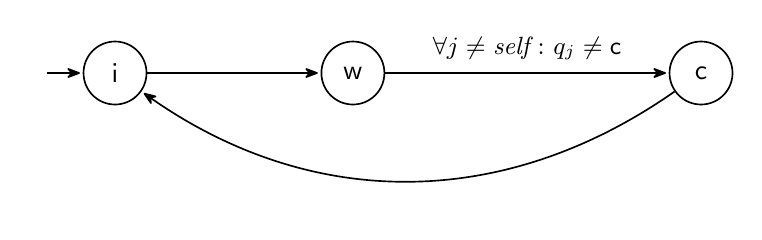
\begin{tikzpicture}[->,>={Stealth[round]},shorten >=1pt,auto,
    node distance=2.2cm,semithick,
    every state/.style={minimum size=8mm,inner sep=1pt}]
  \node[state,initial,initial text={}] (i) {$\Idle$};
  \node[state] (w) [right=of i] {$\Wait$};
  \node[state] (c) [right=3.6cm of w] {$\Crit$};
  \path (i) edge node {} (w)
        (w) edge node[above=1pt] {\small $\forall j \neq \mathit{self}\colon q_j \neq \Crit$} (c)
        (c) edge[bend left=35] node {} (i);
\end{tikzpicture}
\caption{The process template of the running example. The transition from
$\Wait$ to~$\Crit$ is guarded by a universal condition: it is enabled only if
no other process is in~$\Crit$.}
\label{fig:running}
\end{figure}

Configurations are words over the alphabet $\{\Idle, \Wait, \Crit\}$, and the
initial configurations are the words $\Idle^n$, for $n \geq 1$. The bad
configurations are the words that contain at least two occurrences
of~$\Crit$. For example, the instance of size three can reach
$\Wait\Idle\Wait$ from $\Idle\Idle\Idle$ in two steps, and then move to
$\Crit\Idle\Wait$ and to $\Idle\Idle\Wait$, but it can never reach a
configuration such as $\Crit\Idle\Crit$, since the second process in~$\Wait$
is blocked as long as the first one is in~$\Crit$.

The protocol is safe for every~$n$, and for a human reader this is obvious:
the guard is checked and the state is changed in a single atomic step, so no
process can enter the critical section while another one is there. The
example is therefore not interesting as a verification challenge, but it is
small enough to show how each technique handles the unbounded number of
processes. Realistic protocols, such as Burns' or Szymanski's algorithms,
replace the atomic universal condition by a loop in which a process inspects
the other processes one at a time. Their correctness then depends on subtle
interactions between interleaved inspections, and verifying them is
considerably harder~\cite{ABDR08,AHH16}.

\subsection{Well-Quasi-Orderings and Monotonic Systems}
\label{sec:wqo}

Several techniques in this chapter rely on orderings on configurations that
compare instances of different sizes. A \emph{quasi-ordering} on a set is a
reflexive and transitive relation~$\sqsubseteq$. We say that $\sqsubseteq$ is a
\emph{well-quasi-ordering} (WQO) if every infinite sequence $a_0, a_1, a_2,
\ldots$ contains two elements $a_i$ and $a_j$ with $i < j$ and $a_i \sqsubseteq
a_j$. For words, we use the \emph{subword ordering}. We write $u \preceq v$ if
$u$ can be obtained from~$v$ by deleting letters, that is, if $u$ occurs in~$v$
as a not-necessarily-contiguous subsequence. For example, $\Wait\Crit \preceq
\Wait\Idle\Idle\Crit$. Two classical results provide the WQOs used most often
in parameterized verification. By Dickson's lemma, vectors of natural numbers
of a fixed dimension, ordered componentwise, form a WQO. By Higman's
lemma~\cite{Hig52}, the words over a finite alphabet form a WQO under the
subword ordering. Higman's lemma extends to words over any
well-quasi-ordered alphabet, which makes it possible to combine orderings in a
modular way.

A set~$U$ of configurations is \emph{upward-closed} if it contains, together
with every element~$a$, every element~$b$ with $a \sqsubseteq b$. Symmetrically,
$U$ is \emph{downward-closed} if it contains, together with every element~$b$,
every element~$a$ with $a \sqsubseteq b$. We write $\upc{a}$ for the set of elements larger than or equal to~$a$. In the running
example, the set of bad configurations is upward-closed under the subword
ordering: it is the set $\upc{(\Crit\Crit)}$ of words that contain
$\Crit\Crit$ as a subword. Upward-closed sets play a central role for two
reasons. First, under a WQO, every upward-closed set is determined by its
finitely many minimal elements, which gives a finite representation of an
infinite set. Second, every increasing sequence $U_0 \subseteq U_1 \subseteq
\cdots$ of upward-closed sets eventually stabilizes.

We say that a transition system is \emph{monotonic} with respect to an
ordering~$\sqsubseteq$ on its configurations if larger configurations can
simulate smaller ones: whenever $a$ can move to~$a'$ in one step and $a
\sqsubseteq b$, the configuration~$b$ can move in one step to a
configuration~$b'$ with $a' \sqsubseteq b'$. A \emph{well-structured transition system} is a
transition system that is monotonic with respect to a
WQO~\cite{ACJT96,ACJT00,FS01}. In a well-structured system, the set of
configurations from which an upward-closed set~$U$ can be reached is itself
upward-closed. This set can be computed by \emph{backward reachability}: one
starts from $U_0 = U$ and computes $U_{i+1} = U_i \cup \Pre(U_i)$, where
$\Pre(U_i)$ is the set of immediate predecessors of~$U_i$. Each $U_i$ is
upward-closed and is represented by its minimal elements, and the sequence
stabilizes after finitely many steps. Safety then amounts to checking that
no initial configuration belongs to the limit. The algorithm requires that the
minimal elements of $\Pre(U)$ can be computed from those of~$U$, which is the
case for most models considered in this chapter.

Many parameterized systems are monotonic under the subword ordering. Local
transitions, rendez-vous, broadcast, and existential global conditions do not
depend on the number of other processes in a way that could disable them, so
adding processes preserves the ability to perform them. Universal global
conditions are different. In the running example, the configuration~$\Wait$
can move to~$\Crit$, but the larger configuration $\Wait\Crit$ cannot move its
waiting process, because the added process is in the critical section. The
running example is therefore not monotonic, and neither are most mutual
exclusion protocols. Sections~\ref{sec:cutoff} and~\ref{sec:rmc} describe two
ways of dealing with this: view abstraction, which does not require
monotonicity, and monotonic abstraction, which restores it by
over-approximation.

For systems with a clique topology, a configuration can be represented by a
vector of counters, one for each local state. This \emph{counting abstraction}
is exact when processes are anonymous, and it turns the system into a Petri
net, or equivalently a vector addition system, in which each transition adds a
fixed vector to the current counter values~\cite{GerSis92,Esp98}. Petri nets
are monotonic with respect to the componentwise ordering, which is a WQO by
Dickson's lemma, so their coverability problem, and hence the parameterized
reachability problem for such systems, is decidable. A universal global
condition corresponds to a test that a counter is zero, which Petri nets
cannot express. This is another view of why universal conditions are the main
source of difficulty in the analysis of parameterized systems.

% ═════════════════════════════════════════════════════════════════════════════
\section{Early Foundations}
\label{sec:early}
% ═════════════════════════════════════════════════════════════════════════════

The questions studied in this chapter were first formulated in a body of work
from the late 1980s and 1990s that established both the model and the basic
techniques of parameterized verification. This section reviews that work and
some of its later developments.

\paragraph{Correspondence between instances.}
While the undecidability results of Section~\ref{sec:prelim} showed early on
that a general algorithm cannot exist~\cite{AK86,Suz88}, Browne, Clarke, and
Grumberg~\cite{BCG89} proposed a way of transferring
verification results from small instances to large ones. They introduced an
indexed version of the temporal logic CTL$^*$ without the next-time operator,
together with a notion of \emph{correspondence} between systems of different
sizes that preserves the formulas of this logic. Once a correspondence between
a small instance and all larger instances has been established, model checking
the small instance suffices. Establishing the correspondence requires, in
general, an argument by the user, but the approach anticipates the cutoff
theorems of Section~\ref{sec:cutoff}, in which the transfer from small to large
instances is guaranteed by the structure of the system.

\paragraph{Systems with many processes.}
A foundational formulation considers a system composed of a single control
process together with an unbounded collection of user processes sharing a
common definition, communicating through rendez-vous synchronization in the
style of CCS~\cite{GerSis92}. The central contribution was to show that
reasoning about the entire infinite family can be reduced to a finite analysis:
decision procedures were given for checking whether every process satisfies a
given indexed temporal specification. When all processes are identical, the
procedure runs in time polynomial in the size of the process template; in the
presence of a control process, it runs in doubly exponential time. The
reachability questions arising in the analysis were connected to the theory of
Petri nets and vector addition systems, through the counting abstraction
described in Section~\ref{sec:wqo}: since the user processes are anonymous, it
suffices to record how many of them are in each local state. The question of
whether some user process can reach a given local state becomes the
\emph{coverability} problem for Petri nets, which is decidable and, by the
results of Lipton and Rackoff, \textsc{ExpSpace}-complete~\cite{Rac78,Esp98}.
This early demarcation of the boundary between decidable and undecidable cases,
and of the algebraic structures underlying it, shaped much of the work that
followed.

\paragraph{Induction over the number of processes.}
A second early line of work used induction on the number of processes. Kurshan
and McMillan~\cite{KM89}, and independently Wolper and
Lovinfosse~\cite{WL89}, observed that if a process~$I$ is found such that $I$
\emph{abstracts} a single copy of the template, in a sense that preserves the
properties of interest, and the composition of~$I$ with one more copy is again
abstracted by~$I$, then $I$ abstracts the composition of any number of copies.
The
process~$I$ is then a \emph{network invariant}, and verifying the composition
of~$I$ with a fixed environment is sufficient for all sizes. We return to this
idea in Section~\ref{sec:abstraction}. Clarke, Grumberg, and
Jha~\cite{CGJ97} generalized the setting to families of networks generated by
\emph{network grammars}, using abstraction to make the search for invariants
effective.

A complementary line of work targeted linear networks of arbitrary size and
introduced automata as inductive invariants~\cite{SisGyu99}. A correctness
property is itself specified by an automaton, from which an invariant
automaton is synthesized; an induction on the number of processes then
establishes that the property is preserved as the network grows. The method
was shown to be complete for safety properties. It directly anticipates both
the network-invariant approach of Section~\ref{sec:abstraction} and the regular
model checking framework of Section~\ref{sec:rmc}, in which sets of global
configurations of unbounded width are represented symbolically by finite
automata.

\paragraph{Symmetry.}
A further theme running through this early work is the exploitation of the
symmetry inherent in a population of identical processes. Because the identity
of an individual process is immaterial to the global behavior of the system,
verification can be carried out over equivalence classes of configurations
rather than over configurations themselves~\cite{EmeSis96,CEFJ96,ID96}. Two
configurations are equivalent if one is obtained from the other by permuting
the process indices, and the quotient of the state space under this
equivalence can be exponentially smaller than the original. Symmetry
reduction applies to each instance separately, so it does not by itself solve
the parameterized problem, but it explains why configurations of symmetric
systems can be represented by multisets, and it is the basis of the counting
abstraction above. Combining symmetry with fairness leads to on-the-fly model
checking procedures that keep the explored state space
manageable~\cite{GyuSis97}.

\paragraph{Broadcast protocols and cache coherence.}
Esparza, Finkel, and Mayr~\cite{EFM99} studied \emph{broadcast protocols}, in
which a process can send a message that is received by all other processes in
the same step. Broadcast protocols are an extension of Petri nets, in which a
transition can move all tokens from one place to another. They are
well-structured, so safety properties expressed by upward-closed sets can be
checked by the backward reachability algorithm of Section~\ref{sec:wqo}, while
liveness properties become undecidable. Delzanno~\cite{Del00} applied this
framework to cache coherence protocols. Using the counting abstraction and
symbolic representations based on linear arithmetic constraints, he verified
several coherence protocols automatically for an arbitrary number of caches.
This was one of the first demonstrations that parameterized verification could
handle protocols of practical relevance.

\paragraph{Later developments.}
These ideas have been extended in many directions. Parameterized systems with
pairwise rendez-vous have been analyzed on a range of
topologies~\cite{AKRSV18}. In \emph{asynchronous shared-memory systems}, an
unbounded number of anonymous processes communicate through shared registers
without locks~\cite{EGM16}. In \emph{population protocols}, anonymous agents
interact in pairs to compute a predicate of their initial
states~\cite{AADFP06}, and verifying that a protocol computes the intended
predicate for every population size is a parameterized problem that can be
reduced to problems on Petri nets~\cite{EGLM17}. In \emph{ad hoc networks},
processes communicate by broadcast to their neighbors in an unknown graph; the
problem is undecidable in general, and becomes decidable under restrictions on
the possible topologies~\cite{DSZ10}. A recurring observation in this line of
work is that, when processes are anonymous and any behavior of one process can
be replicated by others, the complexity of parameterized verification is often
much lower than that of Petri net coverability~\cite{Esp14}.

Taken together, these strands form the conceptual foundation on which the
remainder of this chapter builds: finite reductions for synchronizing
populations, induction over the number of processes, automata-based
invariants for linear networks, symmetry reduction for replicated components,
and well-structured models of broadcast.

% ═════════════════════════════════════════════════════════════════════════════
\section{Cutoff Methods and Dynamic Cutoffs}
\label{sec:cutoff}
% ═════════════════════════════════════════════════════════════════════════════

A central idea in parameterized verification is the \emph{cutoff theorem}.
The observation behind it is that, for certain classes of systems, one does
not need to verify infinitely many instances. Instead, it
suffices to verify systems up to some finite bound, the cutoff, and
correctness for all larger instances follows automatically~\cite{EN95,EK00}.

Intuitively, this works because processes in many symmetric systems are
interchangeable. If the behavior of a system with~$n$ processes can be
faithfully represented by a system with at most~$k$ processes (the cutoff),
then verifying the $k$-process system is enough. Cutoff results have been
established for important classes such as token-passing rings, guarded
protocols, and systems where processes communicate in restricted ways. This
section first presents such \emph{static} cutoffs, and then \emph{dynamic}
cutoffs, which are discovered during verification.

\subsection{Static Cutoffs}

We say that a number~$k$ is a \emph{cutoff} for a class of parameterized
systems and properties if, for every system and every property in the class,
the property holds for all instances of the system whenever it holds for all
instances of size at most~$k$. A cutoff theorem reduces parameterized
verification to a finite number of finite-state model checking problems, which
can be solved with standard tools. The cutoff typically depends on the class
of systems, on the number of process indices mentioned in the property, and
sometimes on the size of the process template.

\paragraph{Token rings.}
Emerson and Namjoshi~\cite{EN95} studied rings of identical processes in which
a single token, carrying no data, is passed from each process to its neighbor.
They showed that properties in indexed temporal logic that refer to a fixed
number of processes have a cutoff that is a small constant, independent of the
process template. The reason is that a process in a token ring observes the
rest of the ring only through the arrival and departure of the token, and from
the point of view of a few processes, a large ring behaves like a small one in
which the remaining processes have been merged. The result was later extended
from rings to other network topologies by decomposing a network into small
fragments~\cite{CTTV04}, and the existence of cutoffs for token-passing systems
has been characterized in terms of the topology and the specification
logic~\cite{AJKR14}.

\paragraph{Guarded protocols.}
Emerson and Kahlon~\cite{EK00} considered systems of identical processes whose
transitions are guarded by conditions on the other processes. A guard is
\emph{conjunctive} if it requires all other processes to be in a given set of
local states, and \emph{disjunctive} if it requires at least one other process
to be in such a set. They established cutoffs that grow linearly with the
number of local states of the template. For disjunctive guards, the argument
is a simulation: in a run of a large instance, each guard needs only one
witness, and for each local state that occurs in the run it suffices to keep
one process that reaches this state and then stays there, so that it can serve
as a witness whenever needed. A small instance with these extra processes can
reproduce the behavior of the processes mentioned in the property. For conjunctive guards, the argument uses projection instead:
removing processes can only make a conjunctive guard easier to satisfy, so the
projection of a run of a large instance onto a subset of its processes is a
run of a smaller instance. For safety properties this argument is direct,
while liveness properties require more care, since the projection of a fair
run need not be fair, and deadlocks of the large instance need not appear in
the small one. The cutoffs were later sharpened, and extended to fairness and
deadlock detection~\cite{AJK16}, and specialized cutoff methods were developed
for cache coherence protocols~\cite{EK03}.

The running example of Section~\ref{sec:running} is a guarded protocol: the
transition from~$\Wait$ to~$\Crit$ has the conjunctive guard that all other
processes are in $\Idle$ or~$\Wait$. If two processes are in~$\Crit$ at the
same time in a run of some instance, then the projection of the run onto these
two processes is a run of the instance of size two that violates mutual
exclusion. Checking the instance of size two, which has only nine
configurations, is therefore enough to establish mutual exclusion for all
sizes.

\paragraph{Limitations.}
Static cutoff theorems are attractive because they reduce the problem to
standard model checking. However, the bound~$k$ is fixed ahead of time and must
be established before verification begins. This can be limiting: the cutoff
may be large, difficult to compute, or may not exist at all for systems with
richer interaction patterns or more complex topologies. Moreover, each cutoff
theorem covers a specific class of systems, and a protocol that falls slightly
outside the class, for instance because it combines conjunctive guards with
shared variables, is not covered.

\subsection{Dynamic Cutoffs and View Abstraction}

\emph{Dynamic cutoff methods} address these limitations by allowing the
abstraction boundary to be determined adaptively, during the verification
process itself, rather than fixed in advance. A well-developed technique in
this family is \textbf{view abstraction}~\cite{AHH13,AHH16}.
Rather than committing to a single small representative system upfront, the
method reasons about what a process can \emph{observe} about the rest of the
system, and uses those local observations to construct an on-the-fly
abstraction.

The starting point is to model the global state of an $n$-process system as a
configuration: a word of local process states, as in
Section~\ref{sec:prelim}. A \emph{view} of size~$k$ is a subword of length~$k$
of a configuration, that is, a projection of the configuration onto a subset
of~$k$ processes that preserves their order. Instead of tracking full
configurations (whose length varies with~$n$), the method tracks the set of
all views of size up to~$k$ that are reachable across \emph{any} instance of
the system.

For a given precision parameter $k \in \mathbb{N}$, the framework runs two
procedures in parallel. The first is an \emph{under-approximation}: it
performs concrete reachability analysis on instances of fixed size up to~$k$,
and reports a bug if a bad configuration is found. The second is an
\emph{over-approximation} based on abstract interpretation. We write
$\alpha_k$ for the abstraction function, which maps a configuration to its set
of subwords of size up to~$k$. We write $\gamma_k$ for the corresponding
concretization function, which maps a set of views to the set of all
configurations whose subwords of size up to~$k$ all belong to the given set of
views. A fixpoint $V_k$ is then computed over
views using an abstract post operator. The key soundness property is that the
set of reachable configurations~$R$ satisfies $R \subseteq \gamma_k(V_k)$ for
all~$k$, and the approximation becomes tighter as $k$ grows:
$\gamma_{k+1}(V_{k+1}) \subseteq \gamma_k(V_k)$.

An important observation for the implementation is that the abstract post
operator can be computed using only concrete configurations of size up to $k{+}1$, rather than
the full (infinite) concretization. This is because the witnesses required to
enable a global transition consist of a single extra process; accommodating
one additional process beyond the view size is always sufficient. This makes
the fixpoint computation entirely finite and automatic.

If the over-approximation establishes $\gamma_k(V_k) \cap \Bad = \emptyset$,
the system is declared safe. If the under-approximation finds a reachable bad
configuration, the system is declared unsafe. In either case, the current~$k$
is a \emph{dynamic cutoff}, a point discovered during verification beyond
which the search need not continue. If neither procedure is conclusive, the
precision is increased by incrementing~$k$ and the analysis is repeated.

\paragraph{The running example.}
Consider the running example with $k = 1$. The views of size one are single
local states, and all three local states $\Idle$, $\Wait$, and~$\Crit$ are
reachable. The concretization of this set of views contains every
configuration, including $\Crit\Crit$, so the over-approximation cannot prove
mutual exclusion, and the under-approximation, which only explores the
instance of size one, finds no bug. The precision is therefore increased to $k
= 2$.

With $k = 2$, the analysis starts from the views of the initial
configurations, namely $\Idle$ and $\Idle\Idle$. The abstract post operator
considers the configurations of size at most three whose views are all in the
current set, applies the transitions, and collects the views of the results.
In the first rounds, the transition from $\Idle$ to $\Wait$ produces the views
$\Wait$, $\Idle\Wait$, $\Wait\Idle$, and $\Wait\Wait$, and the transition from
$\Wait$ to $\Crit$ then produces $\Crit$, $\Idle\Crit$, $\Crit\Idle$,
$\Wait\Crit$, and $\Crit\Wait$. The view $\Crit\Crit$ is never produced: to
produce it, a process in~$\Wait$ would have to move to~$\Crit$ in a
configuration of size at most three that already contains a process
in~$\Crit$, and the guard forbids this. The fixpoint~$V_2$ therefore consists
of all words of length at most two except $\Crit\Crit$. Its concretization is
the set of configurations with at most one process in~$\Crit$, which is
disjoint from the bad configurations. The method thus proves mutual exclusion
for all sizes, with dynamic cutoff~$2$.

\paragraph{Termination and applications.}
The procedure is guaranteed to terminate whenever the set of reachable
configurations is downward-closed with respect to the subword ordering, as
defined in Section~\ref{sec:wqo}. It also terminates for \emph{monotonic
systems} in the sense of Section~\ref{sec:wqo} when the bad configurations
form an upward-closed set. In that case, safety depends only on the downward
closure of the reachable set, which is closed under the transitions and is
represented exactly by views of bounded size. Monotonic systems cover a broad
and well-studied class, including lossy channel systems, Petri nets (where the
method solves the coverability problem), and timed Petri nets. The running
example is not monotonic, but its reachable set, the set of configurations
with at most one process in~$\Crit$, is downward-closed, so the procedure
terminates as well. For Burns' mutual exclusion protocol, the method likewise terminates at~$k =
2$: already with two-process views it can be shown that no bad configuration
is reachable for any system size.

View abstraction has been successfully applied to a range of protocols,
including mutual exclusion algorithms such as the fine-grained version of
Szymanski's protocol, a benchmark that, to the knowledge of the authors
of~\cite{AHH16}, had not been verified automatically by other methods, as well as cache coherence protocols and distributed
systems with complex process interactions. The framework extends naturally to
other process topologies such as multisets, rings, and trees, and to settings
where global transitions are not assumed to be atomic~\cite{AHH13,AHH16}.
Further refinements of the abstraction, which take into account the context in
which a process takes a step, have been developed in~\cite{AHH14}.

Other dynamic approaches pursue the same goal by different means. Kaiser,
Kroening, and Wahl~\cite{KKW10} consider programs in which an unbounded number
of threads execute the same code over shared variables. They explore instances
of increasing size and detect, during the exploration, a point beyond which
additional threads cannot reach new local states. Like view abstraction, the
method determines the cutoff from the program at hand instead of from a
general theorem.

Together, static cutoff theorems and dynamic approaches like view abstraction
form a complementary toolkit: static cutoffs offer clean theoretical
guarantees for specific protocol families, while dynamic methods
provide greater flexibility and automation for protocols that fall outside
those families. The idea of reasoning about a parameterized system through
its small instances also reappears in the invisible invariants method of
Section~\ref{sec:deductive} and in the small-model properties of the decidable
logics used by SMT-based tools in Section~\ref{sec:smt}.

% ═════════════════════════════════════════════════════════════════════════════
\section{Regular Model Checking}
\label{sec:rmc}
% ═════════════════════════════════════════════════════════════════════════════

Regular Model Checking (RMC) is a symbolic framework for verifying
parameterized and infinite-state systems by representing both sets of
configurations and transition relations using the theory of regular languages
and finite automata~\cite{KW01,BW98,BJNT00}. The key idea is that regular sets
serve as an efficient symbolic representation of infinite state spaces,
playing a role analogous to that of Binary Decision Diagrams (BDDs) in symbolic
model checking of finite-state systems~\cite{AJNS04,Abd12,Abd21}.

\subsection{The Framework}

In its basic form, RMC represents a system as follows. A \emph{configuration}
is a finite word over a fixed alphabet~$\Sigma$, where each symbol encodes the
local state of one component (a process, a stack element, a channel message,
etc.). Sets of configurations, including the initial set and the set of bad
configurations, are represented as regular languages over~$\Sigma$. The
transition relation is encoded as a \emph{length-preserving finite-state
transducer}~$T$ over pairs $(a, a') \in \Sigma \times \Sigma$: the transducer
reads two words of the same length in parallel, letter by letter, and accepts
the pair $(w, w')$ if and only if the system can move from configuration~$w$
to configuration~$w'$ in one step.

This simple setup already captures a wide variety of models. Parameterized
systems consisting of an arbitrary number of finite-state processes in a
linear or ring topology can be modeled by letting each position in the word
represent one process. Systems operating on unbounded queues, stacks, or
integer variables can similarly be encoded by letting word positions represent
data structure contents. The length-preserving constraint on the transducer is
not a restriction for safety verification: for parameterized systems it simply
means that the number of processes is fixed at the start of a run, while
being arbitrary across runs.

\paragraph{A token-passing example.}
Consider a linear array of processes in which a single token is passed from
left to right. Each process is either holding the token or not holding it. We
write $\Tok$ and~$\NoTok$ for these two local states. The initial configurations are those in which
the leftmost process holds the token, that is, the regular language
$\Tok\NoTok^*$. In one step, the process holding the token passes it to its
right neighbor. Figure~\ref{fig:transducer} shows a transducer~$T$ for this
transition relation. It copies a prefix of processes without the token, then
reads the pair $(\Tok,\NoTok)$ for the process that gives the token away,
followed by the pair $(\NoTok,\Tok)$ for the neighbor that receives it, and
finally copies the remaining processes. The safety property states that
exactly one process holds the token, so the bad configurations form the
regular language of words with no~$\Tok$ or with at least two occurrences
of~$\Tok$.

\begin{figure}[t]
\centering
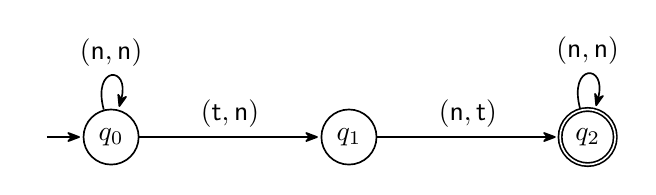
\begin{tikzpicture}[->,>={Stealth[round]},shorten >=1pt,auto,
    node distance=2.3cm,semithick,
    every state/.style={minimum size=7mm,inner sep=1pt}]
  \node[state,initial,initial text={}] (q0) {$q_0$};
  \node[state] (q1) [right=of q0] {$q_1$};
  \node[state,accepting] (q2) [right=of q1] {$q_2$};
  \path (q0) edge[loop above] node {$(\NoTok,\NoTok)$} (q0)
        (q0) edge node {$(\Tok,\NoTok)$} (q1)
        (q1) edge node {$(\NoTok,\Tok)$} (q2)
        (q2) edge[loop above] node {$(\NoTok,\NoTok)$} (q2);
\end{tikzpicture}
\caption{A length-preserving transducer for passing the token one position to
the right. Each transition reads a letter of the current configuration
together with a letter of the next configuration.}
\label{fig:transducer}
\end{figure}

\paragraph{Reachability.}
Let $\Init$ and $\Bad$ be the regular sets of initial and bad
configurations. We write $T^*$ for the reflexive transitive closure of the
transducer relation, and $\Init \circ T^*$ for the set of configurations
reachable from~$\Init$. Safety verification reduces to checking whether
$(\Init \circ T^*) \cap \Bad = \emptyset$. Liveness verification reduces to a
\emph{repeated reachability} problem: checking whether there exists an
infinite computation from~$\Init$ through~$T$ that visits a set of accepting
configurations~$F$ infinitely often.

In the token-passing example, the relation~$T^k$, obtained by composing~$T$
with itself $k$~times, moves the token exactly~$k$ positions to the right, and
each $T^k$ is recognized by a transducer with $k+2$ states. Iterating~$T$ one
step at a time therefore produces an infinite sequence of growing transducers
and never reaches a fixpoint. The transitive closure~$T^+$, however, is
regular: it moves the token any positive number of positions to the right,
and it is recognized by the transducer of Figure~\ref{fig:transducer} with an
additional loop labeled $(\NoTok,\NoTok)$ on the state~$q_1$. The reachable
set is then $\NoTok^*\Tok\NoTok^*$, which is disjoint from the bad
configurations.

\subsection{Computing Transitive Closures}

The central computational challenge is computing $T^+$ (or $\Init \circ
T^*$) effectively. Since the problem is undecidable in general, no method can
succeed on all inputs, and naively iterating the transducer, computing $T^1,
T^2, T^3, \ldots$, does not converge, as the example shows. The standard
approach is to use \emph{acceleration} or \emph{widening} techniques that jump
directly to a representation of~$T^+$.

\paragraph{Acceleration by quotienting.}
Acceleration is typically based on \emph{quotienting}: one finds an
equivalence relation~$\simeq$ on the states of a finite approximation~$T^n$,
merges equivalent states to obtain a quotient transducer $T^n/{\simeq}$, and
checks whether the result characterizes~$T^+$. The difficulty is that
quotienting generally enlarges the accepted language: $L(T^n) \subseteq
L(T^n/{\simeq})$, often strictly. The quotient is therefore taken on the
\emph{history transducer}, a canonical infinite transducer built as the
union of all $T^n$ for $n \geq 1$, where each state records the full sequence
of $T$-states visited during product construction. A key theoretical
contribution is the identification of equivalence relations on the states of
the history transducer whose quotient accepts exactly~$T^+$. Such relations
can be derived from forward and backward bisimulations, and in later work from
simulations, on these states. When the resulting quotient is finite, it is a
transducer for~$T^+$~\cite{AJNO02,AJNO03}. Related constructions iterate
transducers by identifying equivalent states with bisimulation-like
relations~\cite{DLS01}.

\paragraph{Extrapolation and abstraction.}
A different idea is to compute a few iterates $T^1, \ldots, T^k$, detect a
regular pattern of growth between consecutive iterates, and
\emph{extrapolate} it to a guess of the limit, which is then checked for
correctness~\cite{BLW03,BT02}. In the token-passing example, the transducer
for $T^{k+1}$ has one more state, and one more $(\NoTok,\NoTok)$ step between
the pair that gives the token away and the pair that receives it, than the
transducer for~$T^k$. Extrapolation turns this repeated step into the loop
on~$q_1$. \emph{Abstract regular model
checking}~\cite{BHV04} gives up exactness instead: it computes reachable sets
by alternately applying the transducer and abstracting the resulting automata,
for example by merging states that accept the same words up to a given length.
The abstraction guarantees termination, and spurious counterexamples are used
to refine it.

\paragraph{Learning regular invariants.}
For safety verification, it is not necessary to compute the reachable set
exactly: it suffices to find a regular set that contains the initial
configurations, is closed under the transducer, and is disjoint from the bad
configurations. Such a \emph{regular inductive invariant} can be searched for
with techniques from automata learning, in which a learner proposes candidate
automata and a teacher checks the three conditions and returns
counterexamples~\cite{HV05,NJ13,CHLR17}. Checking whether a given automaton is
an inductive invariant is a decidable problem on automata, so the learning
approach replaces the computation of a fixpoint by a sequence of decidable
checks.

\paragraph{Extensions.}
Beyond the linear word model, the framework extends to configurations
represented as trees, enabling verification of systems with hierarchical or
recursive structure~\cite{AJMO02,BT02}. Liveness properties can be handled by
extending the framework to infinite words~\cite{BLW05}, and regular proofs of
liveness have been studied for randomized parameterized systems~\cite{LR16}.
RMC has been successfully applied to token-passing systems, mutual exclusion
algorithms, and systems with unbounded communication channels, stacks, and
integer variables~\cite{AJNS04,Abd12}.

\subsection{Monotonic Abstraction}

While the transducer-based approach is general, it can be
computationally expensive and may not scale to larger protocols. An important
line of work within the RMC framework addresses this by replacing the full
power of regular languages with a lighter symbolic representation based on
\emph{upward-closed sets}, in a technique known as \emph{monotonic
abstraction}~\cite{ADHR07,Abd12}. The approach targets parameterized systems
with a linear process topology and global transitions (both universal and
existential). Configurations are again words over the process state alphabet,
and the subword ordering~$\preceq$ of Section~\ref{sec:wqo} plays a central
role. Bad configurations are characterized by upward-closed sets with respect
to this ordering: if a configuration is bad, then any larger configuration
(with more processes) is also bad. Such sets have a finite symbolic
representation in terms of their minimal elements, making them far more
tractable than arbitrary regular sets.

The core idea is to replace the concrete transition relation~$\to$ with an
abstract relation~$\to_A$ that over-approximates~$\to$ and is monotone with
respect to~$\preceq$. Local and existential transitions are already monotone
and require no approximation. Universal transitions, where a process may
move only if all processes in its context satisfy some condition, are
\emph{not} monotone, since adding more processes to a configuration may
violate the universal condition and disable the transition. The abstraction
handles this by allowing a configuration to silently drop processes that
obstruct the transition, effectively making the universal condition vacuously
satisfiable. Since $\to_A$ is an over-approximation, any safety property
that holds in the abstract model is guaranteed to hold in the concrete one.

Safety verification then proceeds by \emph{backward reachability analysis}, as
in Section~\ref{sec:wqo}. Starting from the upward-closed set $\Bad$ of bad
configurations, one computes the sequence $U_0 = \Bad$, $U_{i+1} = U_i \cup
\Pre_A(U_i)$, where $\Pre_A$ is the predecessor operator under~$\to_A$.
Because $\to_A$ is monotone, each $U_i$ remains upward-closed and can be
represented by a finite set of generators. Termination is guaranteed by
Higman's lemma: the subword ordering~$\preceq$ is a well-quasi-ordering on
words, so every ascending chain of upward-closed sets stabilizes after finitely
many steps. The algorithm terminates when no new generators (up to
subsumption) are produced; if none of the generators represents an initial
configuration, the system is safe.

\paragraph{The running example.}
In the running example, the abstract relation allows a process in~$\Wait$ to
move to~$\Crit$ in any configuration, after deleting the processes that are
in~$\Crit$. For instance, $\Wait\Crit \to_A \Crit$. Backward reachability
starts from the single generator $\Crit\Crit$ and computes the
configurations from which one abstract step leads to a configuration with at
least two processes in~$\Crit$. The steps from $\Idle$ to $\Wait$ and from
$\Crit$ to $\Idle$ do not create processes in~$\Crit$, so a configuration
that reaches $\upc{(\Crit\Crit)}$ by one of these steps already has at least
two processes in~$\Crit$. The abstract step from $\Wait$ to
$\Crit$ deletes all other processes in~$\Crit$, so it always results in a
configuration with exactly one process in~$\Crit$. Hence $\Pre_A$ adds no new
generators, the fixpoint is $\upc{(\Crit\Crit)}$, and since no initial
configuration $\Idle^n$ contains $\Crit\Crit$, the protocol is safe. In this
example the abstraction loses no precision with respect to the property. For
protocols in which a process inspects the others one at a time, such as
Burns' and Szymanski's algorithms, the same approach applies to the
non-atomic versions of the global conditions~\cite{ABDR08}.

\paragraph{Extensions and refinement.}
Monotonic abstraction has been extended to processes with numerical variables
whose values are compared using gap-order constraints~\cite{ADR09}, to tree
topologies, broadcast communication, and binary rendez-vous, and to systems
running under weak memory models (Section~\ref{sec:wmm}). Since the
abstraction may introduce spurious counterexamples, it has been combined with
a counterexample-guided refinement loop that restricts the deletions allowed
in the abstract transitions~\cite{ACDHHR10}. The connection between monotonic
abstraction and well-structured transition systems provides general
decidability results for the abstract systems, for classes of systems that
extend well beyond the purely parameterized setting~\cite{Abd10}.

% ═════════════════════════════════════════════════════════════════════════════
\section{Abstraction and Network Invariants}
\label{sec:abstraction}
% ═════════════════════════════════════════════════════════════════════════════

Abstraction-based methods address the parameterized problem by reducing it to a
finite, non-parameterized one. The idea is to construct an abstract system,
typically a small, fixed-size system, that \emph{over-approximates} the
behavior of the full parameterized family. If a safety property holds in the
abstract system, it holds in all concrete instances~\cite{WL89,PXZ02,ZP04}.
The methods in this section differ in what the abstract system describes: the
environment of a single process, the number of processes in each local state,
or the relationship between a reference process and the others.

\subsection{Network Invariants}

A particularly influential instantiation of this idea is the \emph{network
invariant} method~\cite{WL89,KM89}, further developed
in~\cite{KPSZ02,LHR97}. Consider a system consisting of $n$ copies of a
process template running in parallel. A network invariant is a single
process~$I$ (or small composition of processes) that captures the collective
behavior of all $n-1$ processes that a given process interacts with.
Verifying the property then reduces to checking the two-process composition
of one concrete process with the invariant~$I$, regardless of~$n$. If this
finite system satisfies the property, and~$I$ is a valid over-approximation of
the environment, then all $n$-process instances satisfy it too.

Validity of the invariant is established by induction, as described in
Section~\ref{sec:early}: one checks that $I$ over-approximates a single copy of
the template, and that the composition of~$I$ with one more copy is again
over-approximated by~$I$. Both checks are finite-state problems. The notion of
over-approximation is a preorder on processes, such as trace inclusion or
simulation, that is preserved by parallel composition and that preserves the
properties of interest.

As an illustration, consider the running example from the point of view of
one process. The other processes matter to it only through the question of
whether one of them is in~$\Crit$. A candidate invariant~$I$ has two states,
\emph{free} and \emph{busy}. It can move from free to busy only when the
process it is composed with is not in~$\Crit$, and it can move from busy to
free at any time. The composition of one process with~$I$ satisfies mutual
exclusion, since the process enters~$\Crit$ only when $I$ is free, and $I$
becomes busy only when the process is not in~$\Crit$. The composition of~$I$
with one more process, observed through the same question, behaves again
like~$I$, which establishes validity.

Finding the right invariant automatically is the central challenge. Approaches
range from manual construction guided by domain knowledge, to automated
inference using abstract interpretation, to counterexample-guided abstraction
refinement (CEGAR) adapted to the parameterized setting. In the CEGAR approach,
one begins with a coarse invariant, checks the finite abstract system, and if
a spurious counterexample is found, refines the invariant to rule it out.
Lesens, Halbwachs, and Raymond~\cite{LHR97} compute invariants for linear
networks by iterating the composition and using an approximation that
enforces convergence. Kesten, Pnueli, Shahar, and Zuck~\cite{KPSZ02} developed
a deductive framework for network invariants, based on abstraction relations
between systems, and applied it to a range of examples.

\subsection{Counter Abstraction}

The work of~\cite{PXZ02} combines abstraction with
\emph{$(0,1,\infty)$-counter abstraction}, which tracks for each local state
whether zero, one, or many processes occupy it. Since the number of local
states is finite, the abstract system is finite. Its transitions are
over-approximations of the concrete ones: for instance, when a process leaves
a local state whose counter is~$\infty$, the counter may become either~$1$
or remain~$\infty$.

In the running example, the abstract state is a triple of counter values for
$\Idle$, $\Wait$, and~$\Crit$, and the bad states are those in which the
counter for~$\Crit$ is~$\infty$. A process can enter~$\Crit$ only if the
counter for~$\Crit$ is~$0$, which sets it to~$1$, and leaving~$\Crit$ sets it
back to~$0$. The counter for~$\Crit$ therefore never reaches~$\infty$, and
mutual exclusion holds in the abstract system, which has at most 27 states.

This finite abstraction is often coarse but captures enough structure to
verify mutual exclusion and other coordination properties automatically, and
the abstraction can be systematically refined when needed. The main
contribution of~\cite{PXZ02} concerns liveness. The abstraction loses the
identity of processes, so a fairness requirement for each individual process
cannot be expressed directly. The method adds to the abstract system
fairness conditions derived from the concrete system, which are strong enough
to prove properties such as the absence of starvation.

\subsection{Environment Abstraction}

\emph{Environment abstraction}~\cite{CTV06,CTV08} describes the system from
the point of view of a single reference process. An abstract state consists of
the local state of the reference process together with the truth values of a
fixed set of predicates that describe the other processes in relation to it,
for example whether some process with a smaller index is in its critical
section, or whether some other process holds a message addressed to the
reference process. Because all processes are identical, it suffices to
consider one reference process, and the abstract transition relation can be
computed once from the template. The
approach has been applied to mutual exclusion algorithms, such as the Bakery
and Szymanski protocols, and to cache coherence protocols.

\subsection{Compositional Reasoning for Protocols}

Cache coherence protocols have been a main application of abstraction
methods. McMillan~\cite{McM01} verified the FLASH protocol for an arbitrary
number of processors by compositional model checking, combining symmetry,
case splitting on the involved processors, and abstraction of the remaining
ones, with lemmas supplied by the user. Chou, Mannava, and Park~\cite{CMP04}
turned this approach into a simple and widely used method, often called the
\emph{CMP method}. A few processes are kept concrete, and all others are
replaced by a single abstract process that can perform any action. This
abstraction is usually too coarse, and spurious counterexamples are
eliminated by adding noninterference lemmas, which constrain the actions of
the abstract process and are themselves verified in the abstract model.
Talupur and Tuttle~\cite{TT08} showed that many of the required lemmas can be
derived from the \emph{message flows} of a protocol, the sequences of messages
exchanged to complete a transaction, which designers typically document.

Predicate abstraction has also been lifted to the parameterized setting.
\emph{Indexed predicates} contain free variables that range over process
indices, and the abstraction computes invariants that are universally
quantified over these variables~\cite{LB07}. This makes it possible to infer
properties such as ``for every process~$i$, if $i$ is in its critical section
then the shared lock is held by~$i$''.

\subsection{Thread-Modular Reasoning}

For concurrent programs with an unbounded number of identical threads,
\emph{thread-modular} reasoning verifies a single thread against an
assumption on the effect of the other threads, and checks that each thread
respects this assumption~\cite{FQ03}. Since all threads are identical, a
single assumption serves for all of them, which makes the method naturally
parameterized. The precision of thread-modular reasoning can be increased by
reasoning about~$k$ threads at a time instead of one, which yields a hierarchy
of increasingly precise proof methods~\cite{HMP17}. \emph{Proof
spaces}~\cite{FKP15} provide a related framework, in which correctness proofs
for an unbounded number of threads are built from a finite set of Hoare
triples that are combined using rules that exploit the symmetry of the
threads.

\subsection{Relation to View Abstraction}

The network invariant approach is closely related to view abstraction
(Section~\ref{sec:cutoff}) in spirit: both methods replace the unbounded
environment of a process by a finite abstract summary. The key difference is
in how that summary is constructed and updated. A network invariant is a
single process that must be supplied, or computed and refined, as a separate
object, and its validity is checked by induction; view abstraction
constructs the summary on the fly from the concrete reachability analysis,
refining it incrementally as the precision parameter~$k$ increases. Counter
abstraction and environment abstraction lie in between: the abstract domain is
fixed in advance, but the abstract system is computed automatically from the
template.

% ═════════════════════════════════════════════════════════════════════════════
\section{Deductive and Proof-Based Methods}
\label{sec:deductive}
% ═════════════════════════════════════════════════════════════════════════════

Deductive approaches shift the verification task from automated state-space
exploration to the construction of formal proofs, often assisted by theorem
provers or proof assistants. The idea is to find invariants (properties
that hold at every reachable state of the system for every~$n$) and to prove
that they are preserved by every system transition, regardless of the number
of processes~\cite{OG76,Lam94}. Since the proof is carried out symbolically
over an arbitrary~$n$, this style of reasoning handles unbounded parameters
without requiring enumeration of instances.

\subsection{Inductive Invariants}

We say that a set of configurations is an \emph{inductive invariant} if it
contains all initial configurations and is closed under the transition
relation, that is, every successor of a configuration in the set is again in
the set. An inductive invariant contains all reachable configurations, so if
it is disjoint from the bad configurations, the system is safe. In the
parameterized setting, invariants are expressed as formulas that quantify
over process indices, and the checks are carried out for an arbitrary
number~$n$ of processes.

For the running example, mutual exclusion is expressed by the formula stating
that for all distinct indices~$i$ and~$j$, processes~$i$ and~$j$ are not both
in~$\Crit$. This formula is itself an inductive invariant. It holds initially,
since all processes are in~$\Idle$. A step from~$\Idle$ to~$\Wait$ or
from~$\Crit$ to~$\Idle$ does not create a process in~$\Crit$. A step in which
some process~$k$ moves from~$\Wait$ to~$\Crit$ is only enabled when no other
process is in~$\Crit$, so after the step, $k$ is the only process in~$\Crit$.
The argument does not depend on~$n$ or on~$k$, and it is therefore a proof for
all instances at once.

In realistic protocols, the property to be proved is rarely inductive by
itself. If the universal guard of the running example is replaced by a loop in
which a process checks the other processes one at a time, then a process may
have checked some of the others while they were outside the critical section,
and these processes may have entered it since. The property must then be
\emph{strengthened} with auxiliary assertions, for instance relating the
progress of a process through its loop to the states of the processes it has
already checked. Finding such strengthenings is the creative part of a
deductive proof, and it is the step that the techniques in the rest of this
section, and in Section~\ref{sec:smt}, try to automate.

\subsection{Assertional Reasoning and TLA+}

Classic work by Owicki and Gries~\cite{OG76} laid the groundwork for
assertional reasoning about concurrent programs: each process is annotated
with pre- and post-conditions, and an interference freedom check ensures that
no process's execution invalidates another's assertions. The method was
designed for a fixed, known number of processes, but the underlying proof
discipline (inductive invariants together with noninterference) scales
naturally to the parameterized case by carrying out the annotation and check for a
symbolic, arbitrary process in a family.

Lamport's Temporal Logic of Actions~\cite{Lam94} and the specification
language TLA+~\cite{Lam02} provide a formal language for specifying and proving
properties of concurrent and distributed systems in this spirit. A system is
described by an initial predicate and a next-state relation, and parameters
such as the set of processes are left as constants of the specification. The
TLA+ proof system~\cite{CDLMRV12} supports machine-checked proofs of
invariants for all values of these constants, while the TLC model checker is
used to check the same specification for small, fixed values. Checking small
instances with TLC has proved effective in finding subtle errors in
industrial-scale protocols, for instance at Amazon Web
Services~\cite{NRZBMD15}, and machine-checked proofs extend such results to
all values of the parameters.

\subsection{Invisible Invariants}

A significant challenge for deductive methods is the discovery of inductive
invariants: properties strong enough to be preserved under all transitions and
to imply the desired safety property, but not so strong that they exclude
reachable configurations.
The \emph{invisible invariants} technique of Pnueli, Ruah, and
Zuck~\cite{PRZ01,APRXZ01} addresses this by automatically generating candidate
invariants from small finite instances of the system and then checking whether
they hold inductively for all~$n$. The idea is that the right invariant is
often already visible in small instances and can be generalized to the full
parameterized family.

The procedure works as follows. First, the set of reachable configurations of
an instance of a small size is computed symbolically, for example with BDDs.
Second, this set is projected onto one or two processes, which yields a
formula $\psi(i)$ or $\psi(i,j)$ describing the possible combinations of local
states of these processes. Third, the formula is generalized to the candidate
invariant ``for all~$i$, $\psi(i)$'' or ``for all distinct~$i$ and~$j$,
$\psi(i,j)$''. Finally, the candidate is checked to be inductive and to imply
the property. For a restricted class of systems, the last check can itself be
carried out on an instance of bounded size, by a \emph{small-model theorem}
that bounds the size of a counterexample to inductiveness. In that case the
whole procedure is automatic, and the invariant never needs to be seen by the
user, which explains the name~\cite{ZP04}.

In the running example, the reachable configurations of the instance of size
two, projected onto both processes, give the formula $\psi(i,j)$ stating that
$i$ and~$j$ are not both in~$\Crit$. Its generalization is the invariant from
the beginning of this section. This makes deductive verification partly
automatic, at the cost of completeness: if the right invariant is not among
those generated, the procedure does not terminate with a proof.

\subsection{Interactive Proofs}

More recent work integrates deductive reasoning with interactive tools,
allowing arbitrarily complex invariants to be stated and verified with
machine-checked proofs. The Ivy system~\cite{PMPSS16}, which we return to in
Section~\ref{sec:smt}, is representative of this direction. A
\emph{counterexample to induction} for a candidate invariant is a
configuration that satisfies the candidate but has a successor that does not.
When a candidate invariant is not inductive, Ivy presents such a
counterexample. The user generalizes this configuration into a pattern that should be
excluded, and the tool adds the corresponding conjunct to the invariant. The
checks are carried out automatically, so the interaction focuses on the
insight that the user brings, namely which features of a counterexample
explain why it is unreachable.

Proof-based methods tend to be the most expressive and general of all
approaches to parameterized verification, capable of handling protocols with
complex data structures, arithmetic, and dynamic topology. Their principal
limitation is the burden they place on the user: finding and expressing the
right invariant requires deep insight into the protocol's correctness
argument, and scaling to large or complex protocols remains demanding even
with modern tool support.

% ═════════════════════════════════════════════════════════════════════════════
\section{SMT-Based Methods}
\label{sec:smt}
% ═════════════════════════════════════════════════════════════════════════════

The rise of powerful Satisfiability Modulo Theories (SMT) solvers over the
past two decades has opened new avenues for parameterized verification.
SMT-based methods encode system states, transitions, and properties as logical
formulas and use highly optimized solvers to reason about them
automatically~\cite{BSST09}. Their main advantage over purely deductive
approaches is that the invariant search is largely automated; their main
advantage over finite-state model checking is that sets of states are
represented by formulas over rich theories, which makes them applicable to
systems with rich data and large process counts.

\subsection{Array-Based Systems}

In \emph{array-based systems}~\cite{GR10,GS10}, the parameterized state is
modeled as a collection of arrays indexed by process identifiers, and
quantified formulas express properties over all processes simultaneously. For
the running example, a single array~$s$ maps each process index to its local
state. The initial condition is the formula stating that for every index~$i$,
$s[i] = \Idle$. The transition from~$\Wait$ to~$\Crit$ is described by a
formula stating that there is an index~$k$ with $s[k] = \Wait$, that every
index $j \neq k$ satisfies $s[j] \neq \Crit$, and that the new array is
obtained from~$s$ by setting $s[k]$ to~$\Crit$. The bad configurations are
described by the formula stating that there are two distinct indices $i$
and~$j$ with $s[i] = \Crit$ and $s[j] = \Crit$.

The MCMT tool~\cite{GS10} implements model checking for array-based systems
via backward reachability in a quantified fragment of first-order logic, using
SMT solvers to discharge the fixpoint conditions. The sets of configurations
encountered during backward reachability are represented by existentially
quantified formulas, such as the formula for the bad configurations above. The
predecessors of such a formula are again existentially quantified, provided
that universal guards are handled appropriately; a common treatment
instantiates the universal quantifier only with the indices mentioned in the
formula, which over-approximates the system in a way that closely corresponds
to monotonic abstraction (Section~\ref{sec:rmc}). The test that a new formula
adds no configurations to those already found reduces to the satisfiability of
a formula with an $\exists^*\forall^*$ quantifier prefix, which SMT solvers
handle by instantiation.

In the running example, backward reachability starts from the formula for the
bad configurations. A step from~$\Wait$ to~$\Crit$ by some process~$k$ can
only lead to a bad configuration if the other process in~$\Crit$ was already
there before the step, which contradicts the guard. The other transitions
lead from a configuration to a bad one only if the configuration is itself
bad. The fixpoint is therefore reached immediately, and since no initial
configuration satisfies the formula, the system is safe.

This approach handles systems in which each process has a local state drawn
from an arbitrary (possibly infinite) domain, modeled as an interpreted theory
in the SMT solver. Termination of backward reachability is not guaranteed in
general, but it is guaranteed for classes of systems in which the models of
the existential formulas, viewed as finite structures, are well-quasi-ordered,
which connects the approach to the theory of Section~\ref{sec:wqo}~\cite{GR10}.
The Cubicle model checker~\cite{CGKMZ12} follows the same principles, with a
parallel implementation and a technique that uses finite instances of the
system to guess approximations of the reachable states, with backtracking
when an approximation turns out to be too coarse~\cite{CGKMZ13}. Array-based
methods have seen success on cache coherence and distributed protocols, and
have connections to the decidable array property fragments studied in program
verification~\cite{BMS06}.

\subsection{IC3/PDR and Quantified Invariants}

A prominent line of work in this space is \emph{IC3/PDR} (Property Directed
Reachability), originally developed for finite-state hardware
verification~\cite{Bra11,EMB11} and later extended to the parameterized
setting through quantified invariant inference. IC3/PDR works by incrementally
constructing an inductive strengthening of the safety property. It maintains
a sequence of formulas that over-approximate the sets of states reachable
within increasing numbers of steps. It strengthens these formulas by blocking
states from which a bad state can be reached, propagates facts from each
formula to the next, and stops when two consecutive formulas coincide, at
which point they form an inductive invariant.
In the parameterized setting, these formulas are universally quantified over
process identifiers, and SMT reasoning over the resulting quantified theories
replaces the finite propositional checks of the original algorithm.

Karbyshev et al.~\cite{KBIRS17} developed a variant of PDR that infers
universally quantified invariants. The \emph{diagram} of a state is an
existential formula that describes the state up to the identity of its
elements. When a state must be blocked, the algorithm blocks its diagram.
Blocking a diagram excludes the state together with all larger states that
contain it, which makes the method similar to backward reachability over
upward-closed sets. When it terminates, the algorithm returns a
counterexample, a universal inductive invariant, or a proof that no such
invariant exists.
Gurfinkel, Shoham, and Meshman~\cite{GSM16} exploit the symmetry of
parameterized systems to reduce the inference of quantified invariants to the
inference of invariants for a small number of representative processes, a task
that can be delegated to an SMT-based model checker.

\subsection{Decidable Logics and Ivy}

Tools such as Ivy~\cite{PMPSS16} build on these ideas to provide interactive and automated frameworks for specifying and verifying
distributed protocols. Ivy allows users to specify systems in a first-order
language and restricts the verification conditions to the \emph{effectively
propositional} fragment EPR, in which formulas have a quantifier prefix of the
form $\exists^*\forall^*$ and contain no function symbols, extended with
function symbols whose use satisfies an acyclicity condition. Satisfiability
in this fragment is decidable, and every satisfiable formula has
a finite model whose size is bounded by the formula. Consequently, every
failed check yields a small, finite counterexample, which the user can
inspect, as described in Section~\ref{sec:deductive}. The bound on the size
of models plays a role similar to a cutoff: it limits the number of processes,
messages, and values that need to be considered.

Many protocols do not fit into EPR directly. Padon et al.~\cite{PLSS17}
showed that complex consensus protocols, including several variants of Paxos,
can be verified within EPR by introducing derived relations that keep the
verification conditions in the decidable fragment. In practice, this workflow has successfully verified a range of
distributed protocols, including variants of Paxos, two-phase commit, and
leader election. The inference of invariants for such protocols has also been
automated. One approach generalizes invariants of small finite instances to
quantified invariants and checks them for all sizes~\cite{MGJKKS19}, in the
spirit of invisible invariants; another searches for quantified formulas that
separate reachable states from states that lead to an error~\cite{KPIA20}.

\subsection{Threshold-Based Distributed Algorithms}

Fault-tolerant distributed algorithms form a further class of parameterized
systems, in which the parameters include not only the number~$n$ of processes
but also an upper bound~$t$ on the number of faulty processes. Processes
typically wait until they have received messages from more than a threshold
of other processes, such as $(n+t)/2$, before taking a step. Such algorithms were first
verified by abstraction-based parameterized model checking~\cite{JKSVW13},
and have since been modeled as \emph{threshold automata}, in which
transitions are guarded by linear constraints over message counters and
parameters~\cite{KVW17}. A key result is a \emph{short counterexample
property}: if a threshold automaton violates a safety or liveness property for
some values of the parameters, then it does so in a run whose length, measured
in a suitable sense, is bounded independently of the parameters. Bounded model
checking with an SMT solver over the parameters then suffices for all
parameter values~\cite{KVW17,KLVW17}.

\subsection{Discussion}

The relationship between SMT-based methods and the other approaches in this
chapter is instructive. SMT methods can be seen as automating the invariant
discovery step that deductive methods (Section~\ref{sec:deductive}) leave to
the user, while using a logical representation of state that complements the
regular-language and upward-closed-set representations of
Section~\ref{sec:rmc}: logical formulas easily
express data and arithmetic, while automata easily express the ordering of
processes in a configuration. The tradeoff is decidability: the quantified
theories used by SMT-based tools are generally undecidable, and the tools rely
on heuristics, user interaction, or restriction to decidable fragments to
terminate. SMT-based methods are thus more automatic than purely deductive
approaches, but they lack the termination guarantees of cutoff and monotonic
abstraction methods.

% ═════════════════════════════════════════════════════════════════════════════
\section{Applications to Weak Memory Models}
\label{sec:wmm}
% ═════════════════════════════════════════════════════════════════════════════

Modern multiprocessor architectures do not guarantee Sequential Consistency
(SC)~\cite{Lam79}: for performance reasons, processors reorder memory
operations in ways that are invisible to a single thread but observable
between concurrently executing threads. The resulting \emph{weak} (or
\emph{relaxed}) \emph{memory models} (WMMs) include Total Store Order (TSO),
which underlies x86 and SPARC processors~\cite{OSS09,SSONM10}, and Partial
Store Order (PSO), among others~\cite{AMT14}. Verifying concurrent programs
under such models is substantially harder than under SC, because each thread
is equipped with a buffer that decouples writes from their visibility to other
threads, making the state space infinite even for finite-state programs.
Parameterized verification under WMMs is harder still: one must reason
simultaneously about an unbounded number of threads, each carrying an
unbounded buffer.

Parameterized questions arise naturally in this setting. Synchronization
primitives, such as locks, barriers, and mutual exclusion protocols, are
written to be used by any number of threads, and the same code is executed by
all of them. A correct implementation must work for every number of threads,
and on every architecture on which it is deployed, which means under the
memory model of that architecture.

The connection to the techniques covered in earlier sections is direct.
Backward reachability (Section~\ref{sec:wqo}) applies when the system's
transition relation is monotone with respect to a suitable
well-quasi-ordering on configurations, and monotonic abstraction
(Section~\ref{sec:rmc}) enforces monotonicity by over-approximation when it
does not hold. The key contribution of the weak-memory line of work is to identify the right
semantics and the right ordering to make this apply, even though store and
load buffers introduce data that naively breaks monotonicity.

\subsection{The TSO Model and the Dual Semantics}

Under the classical TSO semantics, each thread is equipped with an unbounded
perfect FIFO \emph{store buffer}. When a thread writes to a variable, the
write is appended to its store buffer rather than committed to memory
immediately; values propagate to shared memory non-deterministically in FIFO
order. A thread reading a variable first checks its own buffer for the most
recent pending write, and falls back to main memory if none is found. Fence
instructions force the buffer to drain before execution continues.

\begin{figure}[t]
\centering
\begin{tabular}{l@{\hspace{3em}}l}
\toprule
Thread 1 & Thread 2 \\
\midrule
$x := 1$ & $y := 1$ \\
$r_1 := y$ & $r_2 := x$ \\
\bottomrule
\end{tabular}
\caption{The store buffering program. The variables $x$ and~$y$ are initially
$0$. Under SC, at least one of the two reads returns~$1$. Under TSO, both reads
may return~$0$.}
\label{fig:sb}
\end{figure}

The program of Figure~\ref{fig:sb} illustrates the difference from SC. Under
SC, one of the two writes is executed first, so at least one of the reads
returns the value~$1$. Under TSO, thread~1 can place its write to~$x$ in its
store buffer, and thread~2 can do the same with its write to~$y$. Each thread
then reads the other variable from memory, where it still has the value~$0$,
so the read of~$y$ by thread~1 returns~$0$, and the read of~$x$ by thread~2
returns~$0$. Only afterwards are the two writes propagated to memory. This
behavior breaks mutual exclusion protocols such as Dekker's and Peterson's
algorithms, which rely on the fact that a thread that has announced its
intention by a write will be seen by the others. Fences are needed to restore
correctness, and verification under TSO is used, among other things, to check
that enough fences have been inserted. We say that a program is
\emph{robust} if all its behaviors under TSO are also possible under SC.
Checking robustness is a related verification problem~\cite{BDM13}.

Decidability of safety verification under TSO for a fixed number of threads
was established by encoding store buffers as lossy channels and applying the
theory of well-structured transition systems (WSTS)~\cite{ABBM10}. However,
these encodings are complex: each channel message must carry a full memory
snapshot, and the reduction involves non-deterministic guessing that leads to
significant state-space explosion in practice.

An alternative approach introduces a \emph{dual} semantics for
TSO~\cite{AABN16,AABN18}. Rather than store buffers, the dual model
equips each thread with a \emph{load buffer}: values propagate
non-deterministically from shared memory into load buffers, and reads are
served from the head of the load buffer rather than from memory directly.
Writes, in contrast, are committed to memory immediately and tagged in the
buffer as \emph{own} messages. In the program of Figure~\ref{fig:sb}, the
initial values of $x$ and~$y$ can propagate into the load buffers of
threads~2 and~1, respectively, before any write takes place. Both writes are
then committed to memory, and each thread reads the old value~$0$ from its
load buffer. Thus, instead of delaying the writes, the dual semantics delays
the reads. The dual semantics is provably equivalent to the classical one, in
the sense that the two models reach the same sets of local states. It offers
significant practical advantages. Because load buffers behave as lossy channels in a
straightforward sense, the WSTS framework applies with far less overhead than
in the store-buffer encoding, yielding a simpler decidability proof and a more
efficient verification algorithm.

\subsection{Parameterized Verification under TSO}

The dual-semantics approach extends naturally to parameterized verification.
In the parameterized setting, the number of threads is a free parameter, and
one asks whether a bad local state is reachable for \emph{any} number of
threads. Parameterized configurations are ordered by a well-quasi-ordering
that combines the subword ordering on load buffer contents with a matching on
threads, in which each thread of the smaller configuration is mapped to a
distinct thread of the larger one; the transition system is shown to be
monotone with respect to this ordering; and backward reachability over
upward-closed sets of configurations terminates by Higman's lemma. This yields
the first decidability result for parameterized verification of concurrent
programs under a weak memory model~\cite{AABN16,AABN18}. Moreover, experiments
with a prototype tool show that parameterized verification is often
\emph{more} efficient than bounding the number of threads to a concrete
value: the sets of minimal elements produced by the backward analysis are
typically much smaller than the configuration sets generated by
bounded-instance analyses. Already for a fixed number of threads, the
load-buffer semantics gives large gains in efficiency and scalability compared
with verification tools based on the store-buffer semantics, on standard mutual
exclusion and memory-model benchmarks~\cite{AABN18}.

The observation that load buffers, unlike store buffers, are compatible with
monotonicity is the central point. Adding a message to a store buffer can
change the value that its thread reads, since the thread reads its own most
recent write, and can therefore disable a transition. Adding a message to a
load buffer only adds the possibility of reading an old value, which the
thread is free to skip. Larger configurations can thus simulate smaller ones,
as required by the theory of Section~\ref{sec:wqo}.

\paragraph{Complexity of parameterized TSO verification.}
While the dual-semantics approach establishes decidability, it leaves open
the precise computational complexity of parameterized TSO verification. This
question was settled in~\cite{AAR20}, where it is shown that the reachability
problem for a parameterized system of identical processes under TSO is
\textsc{PSpace}-complete.

The \textsc{PSpace} upper bound is obtained by combining the load-buffer
(dual) semantics with a careful observation about what information needs to be
tracked: it suffices to maintain, for each process, the set of write
operations it has issued together with the current value it observes for each
variable, rather than the full buffer contents. This yields a polynomial-space
abstraction that is both sound and complete for reachability. The matching
lower bound is established by a reduction from the reachability problem for
1-safe Petri nets, and the reduction relies on the ability of
processes to read the \emph{initial values} of variables from memory. This
dependence on initial values is not merely an artifact of the proof: when
processes are forbidden from reading initial memory values, the reachability
problem drops to polynomial time, since the relevant information can be
captured by a polynomial-sized abstraction tracking only the set of writes
issued across all processes. A further variant is studied in which processes
may perform \emph{atomic read-modify-write} (RMW) operations; it is shown
that adding RMW makes the problem non-primitive recursive,
matching the known hardness of reachability for general lossy channel systems.
Together, these results give a precise and tight complexity picture for
parameterized TSO verification across different fragments of the model.
Parameterized verification has also been studied for other memory models; for
instance, it is \textsc{PSpace}-complete under the release-acquire semantics
of C11~\cite{KGMC22}.

\subsection{The Intel x86 (eTSO) Model}

Real Intel x86 processors implement a memory model that goes beyond TSO. The
formal model eTSO~\cite{RMV22} accounts for multiple memory types, namely
write-back (wb), write-combining (wc), and strong-uncacheable, as well as
non-temporal writes (ntw). Write-back writes behave as in TSO, while
non-temporal writes on different variables may overtake one another, similarly
to PSO. This makes eTSO strictly more relaxed than TSO, and the interaction
between wb and ntw operations introduces subtle orderings that do not arise in
either TSO or PSO alone. Reachability under eTSO for a fixed number of
threads is in general undecidable, but decidability can be recovered by
bounding the number of \emph{alternations} between wb and ntw write stages
per thread~\cite{AABKS24}. A run is $k$-alternation bounded if the writes of
each thread can be partitioned into at most $k$ blocks, alternating between
blocks containing only wb writes and blocks containing only ntw writes. Even
under this restriction, executions may involve unbounded sequences of
operations within each block, and complex shuffles of writes across blocks are
permitted.

Parameterized verification of this $k$-alternation bounded problem was
established in~\cite{AABKS26}. The proof introduces a new transition system,
called the \emph{NTWLoad} system, which combines the load-buffer technique
from the dual TSO semantics (to handle wb writes while preserving monotonicity)
with per-variable store buffers for ntw writes. Each eTSO thread is simulated
by $2k$ concurrent \emph{stage threads}, alternating between wb and ntw
stages, with a finite interface that enforces the required causal dependencies
across stages.

A central technical difficulty is, as explained above, that TSO store buffers
are not monotone with respect to the subword ordering. This difficulty is circumvented by switching wb writes to the
load-buffer representation, in which monotonicity is restored, while ntw
writes retain their store-buffer treatment. The causal dependencies across
stages are maintained through an explicit bookkeeping mechanism. For each
stage, it tracks speculated write values, expected termination labels, and
obligations that must be discharged during execution.

This bookkeeping mechanism introduces a further complication: the resulting
ordering on configurations is not merely a well-quasi-ordering (WQO) but must
be a \emph{better quasi-ordering} (BQO)~\cite{Mar94}. BQOs are strictly
stronger than WQOs and enjoy additional closure properties, in particular
under the powerset construction, that WQOs do not. The ordering on NTWLoad
configurations is built by combining a subword ordering on buffer contents
with an equality constraint on stage information and a powerset-style matching
on thread sets; showing this composite ordering is a BQO requires appealing to
the closure of BQOs under products, word embeddings, and powerset operations.
The transition relation is then shown to be monotone with respect to this BQO,
placing the system within the WSTS framework and yielding decidability of
backward reachability. BQOs had earlier been used in verification to obtain
efficient symbolic representations for timed Petri nets~\cite{AN00,Abd10}. To
the best of our knowledge, the result of~\cite{AABKS26} is the first
application of BQO-based well-structured systems to prove decidability of a
program verification problem.

% ═════════════════════════════════════════════════════════════════════════════
\section{Parameterized Verification of Quantum Circuits}
\label{sec:quantum}
% ═════════════════════════════════════════════════════════════════════════════

The preceding sections have developed parameterized verification in the
classical setting: processes communicate through shared memory or message
passing, the parameter~$n$ counts the number of processes, and correctness
is expressed as a safety or liveness property over an infinite family of
transition systems. A structurally analogous challenge arises in quantum
computing. Most useful quantum algorithms, such as Shor's factoring
algorithm~\cite{Sho97}, Grover's search~\cite{Gro96}, and the Quantum Fourier
Transform, are \emph{parameterized by input size}: a quantum \emph{program}
takes~$n$ as input and dynamically generates the corresponding $n$-qubit
circuit. Verifying such a program requires establishing correctness for all
values of~$n$ simultaneously, a goal that parallels classical parameterized
verification but requires substantially different technical machinery.

\subsection{Quantum States and Circuits}

We recall only the notions needed in this section; a standard introduction
is~\cite{NC10}. The state of~$n$ qubits is a vector of $2^n$ complex
\emph{amplitudes}, one for each \emph{computational basis state}, that is, for
each bit string~$b$ of length~$n$. We write $\ket{b}$ for the basis state that
corresponds to~$b$, and write a state as a sum $\sum_b a_b \ket{b}$, where the
amplitudes~$a_b$ satisfy the normalization condition that the squares of their
absolute values sum to one. A \emph{gate} applies a unitary transformation to
one or a few qubits. The Hadamard gate~$H$ maps $\ket{0}$ to $(\ket{0} +
\ket{1})/\sqrt{2}$ and $\ket{1}$ to $(\ket{0} - \ket{1})/\sqrt{2}$. The
controlled-not gate CNOT acts on a control qubit and a target qubit, and
flips the target if the control is~$1$. A \emph{circuit} is a sequence of
gates, and its effect on a state is the composition of the effects of its
gates.

As a running example for this section, consider the parameterized program
that prepares the \emph{GHZ state} on $n$ qubits. Starting from the state
$\ket{0^n}$, in which all qubits are~$0$, it applies $H$ to the first qubit
and then, for each~$i$ from~$1$ to~$n-1$, a CNOT with control~$i$ and
target~$i+1$. The result is the state $(\ket{0^n} + \ket{1^n})/\sqrt{2}$, in
which all qubits are~$0$ or all are~$1$, each with probability one half.
Figure~\ref{fig:ghz} shows the circuit for $n = 3$.

\begin{figure}[t]
\centering
\begin{minipage}{0.48\linewidth}
\centering
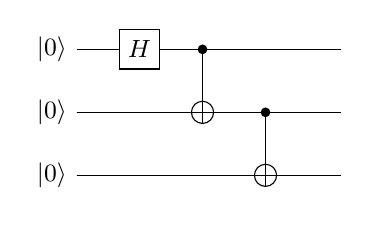
\begin{tikzpicture}[scale=0.8, every node/.style={font=\small}]
  \foreach \y/\l in {0/1, -1/2, -2/3} {
    \draw (0,\y) -- (4.2,\y);
    \node[left] at (0,\y) {$\ket{0}$};
  }
  \node[draw, fill=white, minimum size=5mm, inner sep=0pt] at (1,0) {$H$};
  % CNOT 1 -> 2
  \fill (2,0) circle (2.2pt);
  \draw (2,0) -- (2,-1.18);
  \draw (2,-1) circle (5pt);
  % CNOT 2 -> 3
  \fill (3,-1) circle (2.2pt);
  \draw (3,-1) -- (3,-2.18);
  \draw (3,-2) circle (5pt);
\end{tikzpicture}
\end{minipage}%
\hfill
\begin{minipage}{0.48\linewidth}
\centering
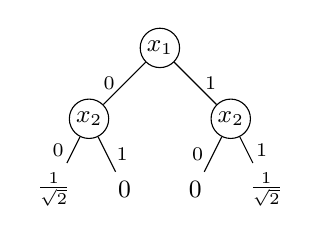
\begin{tikzpicture}[
    level distance=9mm,
    level 1/.style={sibling distance=18mm},
    level 2/.style={sibling distance=9mm},
    every node/.style={font=\small},
    inner/.style={circle, draw, inner sep=1pt, minimum size=5mm}]
  \node[inner] {$x_1$}
    child { node[inner] {$x_2$}
      child { node {$\frac{1}{\sqrt{2}}$} edge from parent node[left, font=\scriptsize] {$0$} }
      child { node {$0$} edge from parent node[right, font=\scriptsize] {$1$} }
      edge from parent node[left, font=\scriptsize] {$0$} }
    child { node[inner] {$x_2$}
      child { node {$0$} edge from parent node[left, font=\scriptsize] {$0$} }
      child { node {$\frac{1}{\sqrt{2}}$} edge from parent node[right, font=\scriptsize] {$1$} }
      edge from parent node[right, font=\scriptsize] {$1$} };
\end{tikzpicture}
\end{minipage}
\caption{Left: the circuit that prepares the GHZ state on three qubits,
consisting of a Hadamard gate followed by two CNOT gates (control marked by a
dot, target by a circle). Right: the GHZ state on two qubits represented as a
binary tree; each path from the root to a leaf selects the values of the
qubits, and the leaf stores the corresponding amplitude.}
\label{fig:ghz}
\end{figure}

\subsection{The Verification Problem}

The correctness criterion for quantum programs is characteristically different
from the safety and liveness properties of
Sections~\ref{sec:early}--\ref{sec:wmm}. Rather than asking whether a bad
state is ever reached, one asks whether the program computes the right
function: given a set of quantum state pairs $(p, q)$, does the program, for
every input size~$n$, correctly map input state~$p$ to output state~$q$? This
\emph{relational} (or \emph{functional}) specification captures input-output
correctness across all parameterized instances simultaneously. For the GHZ
program, the specification consists of the pairs $(\ket{0^n}, (\ket{0^n} +
\ket{1^n})/\sqrt{2})$, one for each~$n$. The specification also subsumes
\emph{equivalence checking} between two parameterized programs, a property of
direct practical importance for verifying that an optimized circuit
implementation is functionally identical to a reference specification,
regardless of~$n$.

Existing approaches to quantum program verification have made notable progress
but fall short of fully automatic treatment of general parameterized circuits.
Deductive approaches, based on quantum Hoare logics~\cite{Yin11} or on proof
assistants in which circuit optimizations are verified once and for
all~\cite{HRHWH21}, can handle parameterized programs but require user
guidance, while symbolic techniques such as path sums~\cite{Amy19}
automatically verify circuits of a fixed size. The Qbricks
project~\cite{Qbricks} develops a deductive framework for circuit-building
quantum programs with rich specifications; it achieves a high degree of
automation, but still requires user-provided annotations such as invariants.
Automata-based approaches~\cite{CCLLTY23,CCLLT23,LSTA25} represent sets of
quantum states by tree automata and compute the effect of each gate
automatically, which makes verification fully automatic for circuits of a
fixed size, and they have been extended to programs with control
flow~\cite{AutoQ20}. A fully automatic framework for general parameterized
quantum programs was an open problem until recently~\cite{AutoQPara}.

\subsection{Representing Infinite Families of Quantum States}

The central challenge in all parameterized verification is finding a finite
symbolic representation of an infinite family of system states, one state
space for each value of~$n$. In the classical setting, regular languages over
a finite alphabet serve this role (Section~\ref{sec:rmc}): a single finite
automaton compactly represents all reachable configurations across all
instance sizes. In the quantum setting, a parameterized program generates an
infinite family of state vectors, one for each~$n$, whose size grows
exponentially with~$n$ but which have a regular recursive structure.

The framework of~\cite{AutoQPara} achieves this through a new automata model
called \emph{synchronized weighted tree automata} (SWTAs). The starting point
is the observation that an $n$-qubit quantum state can be naturally represented
as a binary tree of depth~$n$, as in Figure~\ref{fig:ghz}: each internal node
corresponds to a qubit, and each leaf stores the complex amplitude associated
with a particular computational basis state. Standard tree automata recognize
sets of such trees, providing a symbolic representation of sets of quantum
states that is analogous to finite automata over words. SWTAs extend this with
two additional features. First, \emph{colors} attached to transitions serve as
synchronization labels: all transitions applied at the same level of a tree
must carry the same color, which enforces the level-wise uniformity that
families of quantum states require. A tree is thereby associated with a
sequence of colors, one for each level, and related input and output trees
share the same color sequence; this is the mechanism by which input-output
pairs are linked. Second, \emph{weights} on transitions encode
complex amplitudes, enabling the automaton to represent not merely which
quantum states are possible, but what amplitude each state carries. Together,
these extensions yield a model that defines a \emph{function} from color
sequences to quantum states, rather than simply a set of states. This
functional view is essential for relational verification: it allows a
specification to assert what output state is expected for each input state,
across all input sizes simultaneously.

The GHZ example illustrates the gain in succinctness. The tree for the GHZ
state on $n$ qubits has $2^n$ leaves, but its structure is simple: the left
subtree of the root contains a single nonzero amplitude at its leftmost leaf,
the right subtree contains a single nonzero amplitude at its rightmost leaf,
and all other subtrees are zero. A handful of automaton states, one for each
kind of subtree, describes this structure at every depth, and a weight
of~$1/\sqrt{2}$ at the root gives the amplitudes. The infinite family of GHZ
states, one for each~$n$, is therefore represented by a single small
automaton, in the same way as the infinite family of token-passing
configurations $\NoTok^*\Tok\NoTok^*$ is represented by a small finite
automaton in Section~\ref{sec:rmc}.

\subsection{Transducers for Quantum Gate Semantics}

In regular model checking, the transition relation of a parameterized system
is encoded as a finite-state transducer, and reachability reduces to computing
the transitive closure of that transducer (Section~\ref{sec:rmc}). The quantum
analogue replaces the transition relation with a \emph{quantum gate}, and the
transducer must encode the linear transformation that the gate applies to the
quantum state tree. The framework of~\cite{AutoQPara} introduces a class of
transducers that operate directly on SWTAs: given an input SWTA representing a
family of quantum states, applying a gate transducer produces an output SWTA
representing the family of states after the gate has been applied.

A central concern in any symbolic framework for quantum computation is
\emph{succinctness}: a quantum gate on $n$ qubits is a $2^n \times 2^n$
unitary matrix, and a naive representation is exponential in~$n$. The
transducer representation avoids this blow-up. As an illustration, the
transducer for the Quantum Fourier Transform on $n$ qubits has a number of
states that is \emph{polynomial} in~$n$, exploiting the recursive structure
of the QFT to obtain an exponentially more compact representation than a
matrix encoding would require. This mirrors the advantage of transducers
over explicit transition tables in classical regular model checking.

A further key ingredient is a \emph{composition operator} for transducers.
Given transducers for two sub-circuits, the operator automatically constructs
a transducer for their sequential composition. Starting from transducers for
individual gates, repeated composition assembles the transducer for an
entire circuit without user intervention. The operator extends to
\emph{parameterized programs}: given a transducer for a finite circuit
constituting one layer of a parameterized algorithm, composition generates
a transducer for the full parameterized version with an arbitrary number
of such layers. This step lifts finite-circuit verification to parameterized
verification, and it is the quantum analogue of computing the transitive
closure of a transducer in classical regular model checking.

\subsection{Verification Algorithms and Experimental Results}

With SWTAs as the specification formalism and transducers as the program model,
verification compares the functions from color sequences to quantum states
that SWTAs define. We write $\llbracket \mathcal{A} \rrbracket$ for the
function defined by an SWTA~$\mathcal{A}$. Let $\mathcal{A}$ be the SWTA that
specifies the expected outputs, and let $\mathcal{A}'$ be the SWTA obtained by
applying the program transducer to the input specification. Verification then
reduces to \emph{functional inclusion}, that is, to checking that
$\llbracket \mathcal{A}' \rrbracket$ is contained in $\llbracket \mathcal{A}
\rrbracket$ when both are viewed as sets of pairs of a color sequence and a
state. Equivalence checking between two parameterized programs reduces to
\emph{functional equivalence} of the output SWTAs they produce when applied to
a complete set of linearly independent inputs; correctness of this reduction
follows from the fact that quantum programs implement linear transformations,
so agreement on a complete input basis implies agreement on all inputs.
Functional inclusion and functional equivalence of SWTAs are decidable, and
the framework provides algorithms for both. In contrast, inclusion and
equivalence of the \emph{languages} of SWTAs, viewed as sets of trees, are
undecidable, which is one reason why the functional view is
essential~\cite{AutoQPara}.

The implementation, called \textsc{AutoQ-Para}~\cite{AutoQPara}, was evaluated
on a diverse set of benchmarks spanning algorithmic, arithmetic,
error-correction, and simulation circuits. It successfully verified the
Bernstein-Vazirani algorithm, a ripple-carry adder, a syndrome extraction
circuit from a quantum error-correcting code, and optimized implementations
of Grover's search and Hamiltonian simulation, comparing them against their
unoptimized reference counterparts. Verification times ranged from
14 milliseconds to 11 seconds, and to the best of our knowledge
these are the first fully automatic parameterized verifications of circuits
of this kind.

\subsection{Connections to Classical Parameterized Verification}

The structural parallels with classical parameterized verification are
instructive. In both settings the parameter~$n$ indexes an infinite family of
systems, and the goal is to verify a property of the entire family from a
finite symbolic representation. Regular languages and SWTAs both fill this
role, using words for classical configurations and trees for quantum states.
Transducers encode transition relations in the classical case and gate semantics
in the quantum case, and computing transitive closures or repeated compositions
is the operation that lifts finite reasoning to the parameterized family in
both. The functional inclusion check mirrors the final step of the classical
analyses, amounting to verifying that no reachable output state lies outside
the specification. What distinguishes the quantum setting is the
algebraic structure of the state space: quantum states carry complex amplitudes
subject to normalization and unitarity constraints, and gates are unitary linear
transformations rather than arbitrary relations. The SWTA model is designed to
respect this structure, with weights on transitions as the mechanism for
tracking amplitudes within an automata-theoretic framework. The result can be
seen as an extension of regular model checking to quantum programs, adapted to
the linear-algebraic semantics of quantum computation.

% ═════════════════════════════════════════════════════════════════════════════
\section{Industrial Applications}
\label{sec:industrial}
% ═════════════════════════════════════════════════════════════════════════════

% Placeholder -- to be filled in later.

% ═════════════════════════════════════════════════════════════════════════════
\section{Relations to Other Chapters}
\label{sec:crossrefs}
% ═════════════════════════════════════════════════════════════════════════════

% Placeholder -- cross-references to other chapters in the book to be added later.

% ═════════════════════════════════════════════════════════════════════════════
\section{Conclusion and Open Problems}
\label{sec:conclusion}
% ═════════════════════════════════════════════════════════════════════════════

Parameterized verification asks for guarantees that hold for every number of
components, a question that is undecidable in general. The techniques surveyed
in this chapter respond to this difficulty in different ways, but the same few
ideas recur across all of them: a finite symbolic
representation of infinite families of states, monotonicity with respect to a
well-quasi-ordering, and the observation that the behavior of a large instance
is often already visible in a small one. The applications to weak memory
models and to quantum circuits show that these ideas carry over to settings
that look very different from the protocols for which they were first
developed.

Several problems remain open or only partially solved. Liveness properties
under fairness are much less well supported than safety properties, both in
theory and in tools, since abstractions that preserve safety often lose the
information needed for fairness. For weak memory models, parameterized
verification is well understood for TSO and some of its extensions, but the
more relaxed models of ARM and POWER processors, and the language-level models
of C11 and Java, are only partly covered. For distributed protocols, the
automatic inference of invariants with alternating quantifiers, which are
needed for many consensus protocols, remains difficult, and current tools
handle it by restricting the logic or by relying on the user. In the quantum
setting, the automata-based approach covers parameterized circuits, and its
extension to programs with measurement, classical control, and noise is a
natural next step. Finally, the parameterized view applies to further classes of
systems built from many copies of the same component, such as multi-agent
systems and large-scale distributed services, where the same questions about
correctness for any number of components arise.


% ── Bibliography ──────────────────────────────────────────────────────────────
{\small
\bibliography{refs}
}

\end{document}
